% !TEX encoding = UTF-8 Unicode
%%%%%%%%%%%%%%%%%%%%%%%%%%%%%%%%%%%%%%%%%%%%%%%%%%%%%%%%%%%%%%%%%%%%%%%%%%%%%%%%%%%%%%%%%%%%%%%%%%%%%%% 
%%
%%  This file is asmeconf-template.tex, a LaTeX template to format ASME Conference papers according to
%%  the requirements on ASME's conference web pages, and including hypertext support for the pdf.
%%
%%  This file is version 1.46 dated 2026/01/10
%%  
%%  As of version 1.11, this template defaults to ASME's newer conference guidelines first posted July 2019.
%% 			Those guidelines changed the author block formatting to be inline. 
%%			If you prefer the traditional grid format, use the class option [grid].
%%			Nomenclature now follows the abstract, and the abstract text is set in italics.
%%
%%  Author: John H. Lienhard, V
%%          Department of Mechanical Engineering
%%          Massachusetts Institute of Technology
%%          Cambridge, MA 02139-4307 USA
%%
%%  Class options include:
%%
%%          * An option to use the traditional grid arrangement of author names, [grid].  
%%			*	 With this option, line breaks (\\) may be inserted into the address as needed. 
%%			*	 Author names that include commas should be enclosed in braces, e.g.,  {Joseph L. Smith, Jr.}.  
%%			*	 Authors may be grouped above a single affiliation using braces, e.g., {Henry Tudor, Catherine Parr}.
%%
%%          * An option to balance the heights of columns on the last page, [balance]. 
%%
%%          * An option to include line numbers, [lineno]. You must *run twice* for proper placement of the line numbers. 
%%			*	 The lineno package does not number titles, footnotes, captions, or tables.
%%          *    This option will disable balancing column height on final page if that option has been invoked.
%%          *    The lineno package won't always number the lines preceding displayed math in a paragraph because
%%          *    paragraph has not ended.  See that package's documentation for macros to address this problem, or
%%          *    just leave a blank line above the displayed equation while you are editing and then remove the 
%%          *    blank line along with [lineno] option when you move to your final version.
%%
%%			* An option not to use a boldface font for caption text, [unboldcaption]
%%
%%          * Options to: 	omit the ASME copyright footer, [nofoot]; 
%%			*				use government employee copyright notice,      [govt];
%%			*				use government contractor copyright notice,    [contractor];
%%			*				use copyright notice for some gov't employees, [somegovt];
%%			*				omit the conference headers on the titlepage,  [nohead]
%%
%%			* Option to use LuaLaTeX **without** unicode-math and fontspec, [nofontspec]
%%
%%          * Math options from M. Sharpe's newtxmath package: upright integrals [upint]; 
%%          *    [varvw] for a v and w that are better distinguished from Greek nu; and also 
%%          *    [subscriptcorrection, smallerops, varg, frenchmath, varbb, cmbraces, slantedGreek,...] 
%%			* 	 See newtx documentation for descriptions (at CTAN: https://www.ctan.org/pkg/newtx, v1.744 or higher is best).
%%			*	 newtx is not loaded with lualatex unless the [nofontspec] option is used.
%%
%%          * An option to allow hyphenation of the typewriter font [hyphenate], from the inconsolata package (pdfTeX only).
%%          *    Hyphenation is normally suppressed for a typewriter (monospaced) font because those are often used for code.
%%			*	 To replace the default variable word spacing by monospacing, use the option [mono].
%%			*	 To get a zero without a slash, use [var0]
%%
%%			* PDF/A compliance:  Since 2022, LaTeX has included support for PDF/A, through the \DocumentMetadata{..} command.
%%
%%          * Options (used by the babel package) to include passages in languages other than English (e.g., a translation 
%%			*    of the abstract).  See Appendix C for details.
%%			*    	pdftex: Appropriate scripts will be loaded if you call the class options [greek], [russian], or [vietnamese].
%%			*    
%%			*    	lualatex: Language support is most extensive when running LuaLaTeX, which automatically loads fontspec.
%%			*		Non-Latin scripts require the [loadscripts] option, see Appendix C. 
%%			*	 	Be aware that you might need to install additional fonts for some languages.
%%			 
%%  The use of commands defined or modified by the asmeconf class is illustrated throughout this file. In particular, 
%%  ASME requires capitalized section headings, and as a result some care is needed when using macros in section headings,
%%  as also illustrated below.
%%
%%  Use an **up-to-date and complete** installation of LaTeX, such as TeX Live 2025 or later. 
%%		LaTeX formats earlier than 2022 are not fully supported.
%%
 %=========================================================
%% 
%% LICENSE: 
%%
%% Copyright (c) 2026 John H. Lienhard
%%
%% Offered under the MIT license: https://ctan.org/license/mit 
%%
%%%%%%%%%%%%%%%%%%%%%%%%%%%%%%%%%%%%%%%%%%%%%%%%%%%%%%%%%%%%%%%%%%%%%%%%%%%%%%%%%%%%%%%%%%%%%%%%%%%%%%% 

%%  RECOMMENDED pdf management code.
%%  This code was added to the LaTeX kernel in June 2022.
%% 		See https://www.latex-project.org/news/latex2e-news/ltnews35.pdf
%%  If you have problems with these lines, you can comment them out or, better, update your LaTeX format.

% \DocumentMetadata{
% 	lang		= eng-US, 	% default
% 	pdfstandard	= A-3u,		% A-2b, A-2u, A-3b, A-3u. Check that your figures also meet the standard you choose.
% 	pdfversion	= 1.7, 		% an older version of PDF, but very widely supported
% %	pdfversion  = 2.0, 		% default for LaTeX. Version 2.0 supports tagged PDF.
% %	pdfstandard = { ua-2 , a-4f }, % run with lualatex and use a very recent LaTeX format (e.g., 2025/11/01)
% %	tagging 	= on, 		% for producing tagged pdf
% }

%%%%%%%%%%%%%%%%%%%%%%%%%%%%%%%%%%%%%%%%%%%%%%%%%%%%%%%%%%%%%%%%%%%%%%%%%%%%%%%%%%%%%%%%%%%%%%%%%%%%%%%

%% CLASS OPTIONS are described above. Change the options given below to meet your needs.
%% 
%%	 	NB: Remove the [colorlinks] option before *final* submission to ASME, to get black text for printing,
%%			but keep that option for electronic use.
%%
%%		NB: If you are not using the language options, * remove * them (together with Appendices C and D).
%%			Greek, cyrillic languages, and vietnamese if used, must be named as \documentclass options under pdftex.
%%			Spanish, german, and many others, if used, do not need to be named when the babel package is dated 2024 or later.
%%
%%		NB: the mathalfa option was dropped in v1.41; load the mathalpha package in your preamble instead.

\documentclass[colorlinks,upint,subscriptcorrection,varvw,hyphenate,balance]{asmeconf} % simplified
\usepackage{tikz}
\usetikzlibrary{arrows.meta,patterns,decorations.markings,decorations.pathmorphing,calc}
\usepackage{booktabs}
\usepackage{array}

% Custom commands for beam theory
\newcommand{\dds}{\frac{d}{ds}}
\newcommand{\ddds}{\frac{d}{d\bar{s}}}
\newcommand{\xbar}{\bar{x}}
\newcommand{\ybar}{\bar{y}}
\newcommand{\sbar}{\bar{s}}
\newcommand{\kbar}{\bar{\kappa}}


%\documentclass[colorlinks,upint,subscriptcorrection,varvw,balance,loadscripts,german,vietamese]{asmeconf} % lualatex

%%%%%  pdf metadata  %%%%%%%%%%%%%%%%%%%%%%%%%%%%%%%%%%%%%%%%%%%%%%%%%%%%%%%%%%%%%%%%%%%%%%%%%%%%%%%%%%

\hypersetup{%
	pdfauthor={Hai-Jun Su, Ben Survey},
	pdftitle={Hierarchical Multi-fidelity Modeling Stack for Design and Analysis of Compliant Mechanisms},
	pdfkeywords={compliant mechanisms, multi-fidelity modeling, beam constraint model, pseudo-rigid-body model, finite element analysis, large deflections},
	pdfsubject = {Hierarchical multi-fidelity modeling stack for compliant mechanisms},
}
% If an author name or the title include a comma, enclosed it in braces, e.g., pdfauthor{John Forbes Nash{,} Jr.}


%%%%%%%%%%%%%%%%%%%%%%%%%%%%%%%%%%%%%%%%%%%%%%%%%%%%%%%%%%%%%%%%%%%%%%%%%%%%%%%%%%%%%%%%%%%%%%%%%%%%%%%

\allowdisplaybreaks % from amsmath package, allows multiline equations to break across pages (delete if not wanted)
					% using \\* instead of \\ will prevent specific lines from being pagebreaks.

% logos used in this document
\newcommand*\pdfTeX{pdf\TeX}    
\newcommand*\LuaLaTeX{Lua\LaTeX}
\newcommand*\BibTeX{Bib\TeX}

\begin{document}

% Change these fields to the right content for your conference.
% You can comment these out if for some reason you don't want a header.
% Use title case for the conference name (first letters capitalized), not all capitals

\ConfName{Proc. of the ASME 2026 IDETC/CIE}
\ConfAcronym{IDETC/CIE 2026}
\ConfDate{August 23--26, 2026} 
\ConfCity{Houston, TX}
\PaperNo{DETC2026-XXXXX}

% Units of measure (e.g., cm) and other specialty lowercase terms in the title should be 
%   enclosed in \NoCaseChange{...} to maintain lower case type.
%   The rest of the title will automatically be set in all capital letters.
%
%	\title{Place Title Here: Place Subtitle After Colon} 

\title{Hierarchical Multi-fidelity Modeling Stack for Design and Analysis of Compliant Mechanisms} 
 
%   Put author names into the order you want. Use the same order for affiliations.
%   \affil{#} tags the author's affiliation to the address in \SetAffiliation{#}.
%   No space between last name and \affil{#}, separate names with commas.
%
%	For a sole author or a single affiliation for all authors, {#} may be left empty, i.e. \affil{} and \SetAffiliation{} (but not with [grid] option!)
%
%   \CorrespondingAuthor{email} follows that author's affiliation, no spaces before or after 
%   If multiple corresponding authors, put both email addresses in the same command and place after both authors.
%
%   \JointFirstAuthor, if applicable, follows the affiliation of the relevant authors, no spaces.

\SetAuthors{%
    Hai-Jun Su\affil{1}\CorrespondingAuthor{su.298@osu.edu}, Ben Survey\affil{1}
	}
%	Note: Luis and Maria are not real people.  Henry and Catherine have been dead for >450 years.

\SetAffiliation{1}{Department of Mechanical \& Aerospace Engineering, The Ohio State University, Columbus, Ohio, USA}
%   Note: You can force a line break in the address using \\ 

%	To switch from inline author names to gridded names, use the [grid] option.

\maketitle

\keywords{compliant mechanisms, multi-fidelity modeling, beam constraint model, pseudo-rigid-body model, finite element analysis, large deflections}

\begin{abstract}
This paper presents a hierarchical, eight-level multi-fidelity modeling stack as a general technical routine for the design and analysis of compliant mechanisms, using the parallelogram flexure as a representative case study. Providing a unified framework that bridges the gap between rapid conceptual synthesis and rigorous physical validation, the motivation stems from the fundamental challenge in compliant mechanism design where deep coupling between kinematics and elastomechanics requires designers to balance computational speed with predictive accuracy for large-deflection regimes. Our methodology involves the systematic implementation and cross-validation of modeling levels spanning from first-order linear theory and algebraic models (BCM, PRBM) to exact transcendental solutions (Guided Beam), numerical boundary value problem (BVP) solvers, and high-fidelity 3-D solid finite element analysis (FEA). Major results demonstrate a performance spread of over eight orders of magnitude in computational runtime, while quantifying the divergence of low-order models in predicting parasitic rotations and behavior near buckling thresholds. These findings provide a validated roadmap for designers to select optimal modeling fidelities for various classes of compliant systems, facilitating more efficient and accurate synthesis of high-precision flexures.
\end{abstract}

%%%%%%%%%  BODY OF PAPER %%%%%%%%%%%%%%%%%%%%%%%%%%%%%%%%%

\section{Introduction}
\label{sec:introduction}

Compliant mechanisms (CMs) represent a significant departure from traditional rigid-body kinematics, achieving motion through the elastic deformation of flexible members rather than solely via discrete kinematic pairs \cite{howell2001}. Inspired by the pervasive compliance found in biological systems, these mechanisms offer transformative advantages for high-performance engineering, including the elimination of backlash and friction, reduced part count, and the capability for extreme miniaturization. Consequently, CMs have become indispensable in precision application domains such as nanomanufacturing, optical manipulation stages, and surgico-robotic instruments where traditional joints would introduce impermissible positioning and repeatability errors \cite{handbook2013}.

Despite their advantages, the design and analysis of CMs remain fraught with fundamental challenges that constitute major "open problems" in the field. A primary difficulty is the deep coupling between kinematics and elastomechanics; unlike rigid-body systems where geometry and force can be decoupled, the motion of a CM is an intrinsic function of its instantaneous loading state and material properties. Furthermore, these mechanisms often operate in large-deflection regimes where geometric nonlinearities---such as elastokinematic shortening, load-stiffening, and buckling---dominate behavior. Bridging the gap between conceptual synthesis and high-fidelity physical validation remains a significant hurdle for designers, often resulting in costly prototyping iterations due to a lack of integrated modeling frameworks.

The current state-of-the-art in reduced-order modeling for planar flexures generally spans a spectrum of fidelities, ranging from linear theory to exact analytical solutions. Linear theory provides a rapid baseline for initial stiffness but inherently fails to capture parasitic motions or workspace limits. To address these limitations, Pseudo-Rigid-Body Models (PRBMs) approximate flexible segments as rigid links connected by lumped torsional springs \cite{Howell1994, Howell1995}. While PRBMs are highly effective for conceptual synthesis and large-deflection workspace estimation, they often lack the localized precision required for high-precision flexures and may neglect subtle constraint variations. More advanced variants, such as 3R model \cite{Su2009PRB3R}, have been developed to improve approximation accuracy for large-deflection beams by utilizing multi-link chains. Beam Constraint Models (BCMs) utilize polynomial expansions to capture load-dependent constraints and elastokinematic shortening effects in the intermediate deflection range \cite{awtar2007characteristics, AwtarSen2010}. For extreme deflections or complex composite structures, geometrically exact beam theories (GEBT) provide a robust framework for general nonlinear analysis \cite{Yu2012GEBTAG}. Elliptic integral solutions are considered the most precise analytical method for simple geometries; recent work by Zhang and Chen \cite{zhang2013comprehensive} has provided comprehensive solutions that explicitly handle multiple inflection points and complex loading conditions, though these remain computationally intensive compared to closed-form models.

Bridging the gap between conceptual synthesis and high-fidelity physical validation remains a significant obstacle in compliant mechanism design, often resulting in costly prototyping iterations due to a lack of integrated modeling frameworks. A major challenge lies in the coupling of nonlinear beam governing equations with traditional kinematic constraints; for instance, the presence of pin joints or multiple flexible segments in a complex mechanism leads to a system of equations that is difficult to solve simultaneously without robust initialization. This paper addresses these challenges by presenting a hierarchical, eight-level multi-fidelity modeling stack. While we utilize the parallelogram flexure mechanism as our primary case study, the underlying technical routine is general and applicable to a wide range of compliant topologies. We implement and cross-validate each level---extending from first-order linear solvers to optimized PRBMs, exact nonlinear Boundary Value Problem (BVP) solvers, and 3D solid FEA. By quantifying the trade-offs in computational speed and predictive accuracy, we provide a validated roadmap that allows designers to navigate the full complexity of static and kinematic mechanism design within a unified framework.

% Section 4.3 was moved from here to Section 3.8/4.3 location

\section{Beam Equations}
\label{sec:beam_equations}
In this section, we derive the exact nonlinear governing equations for a single cantilever beam and a fixed-guided beam.

\subsection{Fixed-Free Beam Equations}
Consider a flexible cantilever beam of length $L$, modulus $E$, and inertia $I$. We parameterize the beam by its arc length $s \in [0, L]$. The angle between the beam tangent and the $x$-axis is $\theta(s)$.

\begin{figure}[ht]
\centering
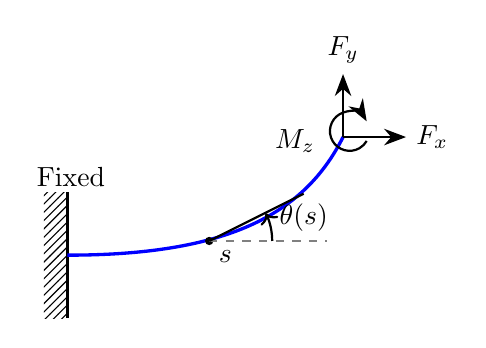
\begin{tikzpicture}[scale=1.0]
    \fill[pattern=north east lines] (-0.3,-0.8) rectangle (0,0.8);
    \draw[very thick] (0,-0.8) -- (0,0.8);
    \draw[very thick, blue] (0,0) .. controls (2,0) and (3,0.5) .. (3.5,1.5);
    \node[left] at (0.6,1) {Fixed};
    \draw[-{Stealth[scale=1.2]}, thick, black] (3.5,1.5) -- (4.3,1.5) node[right] {$F_x$};
    \draw[-{Stealth[scale=1.2]}, thick, black] (3.5,1.5) -- (3.5,2.3) node[above] {$F_y$};
    \draw[{Stealth[scale=1.2]}-, thick, black] (3.8,1.7) arc (30:330:0.25) node[left, xshift=-15pt] {$M_z$};
    % Definition of theta(s) at point s
    \coordinate (P) at (1.8,0.18);
    \fill[black] (P) circle (1.5pt) node[below right] {$s$};
    \draw[dashed, gray] (P) -- ++(1.5,0);
    \draw[thick, black] (P) -- ++(1.2,0.6); % Tangential direction
    \draw[->, thick] ($(P)+(0.8,0)$) arc (0:26:0.8);
    \node at ($(P)+(1.2,0.3)$) {$\theta(s)$};
\end{tikzpicture}
\caption{Cantilever beam under tip loading illustrating kinematic variables}
\label{fig:cantilever}
\end{figure}

The kinematic relations for an inextensible beam are given by the projection of the tangent onto the coordinate axes:
\begin{equation}
\frac{dx}{ds} = \cos\theta, \quad \frac{dy}{ds} = \sin\theta, \quad \kappa(s) = \frac{d\theta}{ds}
\label{eq:kinematic}
\end{equation}
Moment equilibrium and the Euler-Bernoulli constitutive law ($M = EI\kappa$) yield the governing second-order ODE:
\begin{equation}
EI \frac{d^2\theta}{ds^2} = F_x \sin\theta - F_y \cos\theta
\label{eq:governing_dim}
\end{equation}

The dimensional governing equations can be generalized by introducing the dimensionless variables defined in Table~\ref{tab:normalization}. Substituting these into Eq.~\eqref{eq:kinematic} and Eq.~\eqref{eq:governing_dim} yields the normalized second-order ODE:
\begin{equation}
\frac{d^2\theta}{d\sbar^2} = \alpha_x \sin\theta - \alpha_y \cos\theta
\label{eq:normalized_ode}
\end{equation}

\begin{table}[ht]
\centering
\caption{Normalized Variables for Euler Beam}
\label{tab:normalization}
\begin{tabular}{lcl}
\toprule
\textbf{Variable} & \textbf{Definition} & \textbf{Description} \\
\midrule
$\sbar$ & $s/L$ & Norm. arc length $\in [0,1]$ \\
$\xbar, \ybar$ & $x/L, y/L$ & Norm. positions \\
$\kbar$ & $L\kappa$ & Norm. curvature \\
$\alpha_x, \alpha_y$ & $F_x L^2 / EI, F_y L^2 / EI$ & Norm. forces \\
$\beta$ & $M_z L / EI$ & Norm. tip moment \\
\bottomrule
\end{tabular}
\end{table}

The resulting system consists of Eq.~\eqref{eq:normalized_ode} and the normalized kinematic relations $d\xbar/d\sbar = \cos\theta$ and $d\ybar/d\sbar = \sin\theta$. This constitutes a boundary value problem (BVP) with boundary conditions at the fixed end ($\xbar(0)=0, \ybar(0)=0, \theta(0)=0$) and the tip condition ($\theta'(1)=\beta$). This BVP is solved numerically using an iterative BVP solver, such as the shooting method or a collocation-based solver like \textit{solve\_bvp}, to obtain the full beam profile and tip displacement for any given loading $(\alpha_x, \alpha_y, \beta)$. While these numerical solvers are remarkably efficient and provide exact results in terms of beam theory, they are sensitive to the initial guess and can struggle to converge under large buckling forces where more than one equilibrium solution may exist (e.g., higher-order buckling modes). Furthermore, while the BVP approach is fast for individual beams, it is often difficult to couple these equations directly with discrete kinematic constraints, such as pin joints, which are common in hybrid compliant-rigid mechanisms. The Python implementation of this solver is publicly available in our GitHub repository.



\subsection{Fixed-Guided Beam Eequations}
The fixed-guided beam is a variation of the cantilever where the tip is constrained to remain flat ($\theta(1) = 0$). This constraint renders the tip moment $\beta$ an unknown reaction. In normalized form, the problem constitutes an Euler-Bernoulli BVP:
\begin{align}
&\frac{d\mathbf{q}}{d\sbar} = \begin{bmatrix} \cos\theta \\ \sin\theta \\ \kbar \\ \alpha_x \sin\theta - \alpha_y \cos\theta \end{bmatrix}, \quad \mathbf{q} = \begin{bmatrix} \xbar \\ \ybar \\ \theta \\ \kbar \end{bmatrix} \label{eq:guided_bvp} \\
&\text{BCs: } \xbar(0) = \ybar(0) = \theta(0) = 0, \quad \theta(1) = 0
\end{align}
\begin{figure}[ht]
\centering
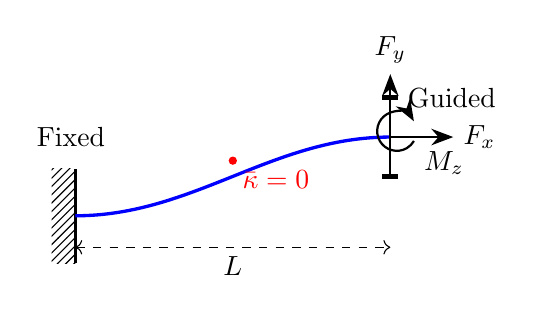
\begin{tikzpicture}[scale=1.0]
    % Ground
    \fill[pattern=north east lines] (-0.3,-0.6) rectangle (0,0.6);
    \draw[very thick] (0,-0.6) -- (0,0.6);
    
    % S-shape beam (symmetric about midpoint)
    \draw[very thick, blue] (0,0) .. controls (1.5,0) and (2.5,1) .. (4,1);
    \node[left] at (0.5,1) {Fixed};
    
    % Inflection point
    \fill[red] (2,0.7) circle (1.5pt) node[below right, red] {$\kbar=0$};
    
    % Guide symbol at tip
    \draw[ultra thick, black] (3.9,0.5) -- (4.1,0.5);
    \draw[ultra thick, black] (3.9,1.5) -- (4.1,1.5);
    \draw[thick, black] (4,0.5) -- (4,1.5);
    \node[right] at (4.1,1.5) {Guided};
    
    % Loading and reaction moment
    \draw[-{Stealth[scale=1.2]}, thick, black] (4,1) -- (4.8,1) node[right] {$F_x$};
    \draw[-{Stealth[scale=1.2]}, thick, black] (4,1) -- (4,1.8) node[above] {$F_y$};
    \draw[{Stealth[scale=1.2]}-, thick, black] (4.3,1.2) arc (30:330:0.25) node[below right] {$M_z$};
    
    % Dimensions
    \draw[<->, dashed] (0,-0.4) -- (4,-0.4) node[midway, below] {$L$};
\end{tikzpicture}
\caption{Fixed-guided beam configuration showing characteristic S-shape deformation and horizontal tip constraint}
\label{fig:fixed_guided}
\end{figure}

A fundamental property of this BVP is the \textit{Curvature Antisymmetry Theorem}:
\begin{equation}
\kbar(\sbar) = -\kbar(1-\sbar) \quad \text{for all } \sbar \in [0,1]
\label{eq:antisymmetry}
\end{equation}
implying an inflection point at the span midpoint ($\kbar(0.5) = 0$). While the curvature $\kbar(\sbar)$ is antisymmetric, the angle $\theta(\sbar)$ is symmetric about the midpoint ($\theta(\sbar) = \theta(1-\sbar)$), reaching its maximum at $\sbar = 0.5$.

This BVP is solved numerically using a collocation method (e.g., \textit{solve\_bvp} in Python or \textit{bvp4c} in MATLAB). To ensure robust convergence, the solver is initialized with a cubic displacement guess consistent with the linear Bernoulli-Euler profile for a guided beam:
\begin{equation}
\ybar_{init}(\sbar) = (3\sbar^2 - 2\sbar^3)\delta_{linear}
\label{eq:init_guess}
\end{equation}
where $\delta_{linear} = \alpha_y/12$. The reaction moment is subsequently extracted as $\beta = \kbar(1)$. The BVP solver for fixed-free and fixed-guided beams has been implemented in a Python script, which is publicly available in our GitHub repository.

\section{Parallelogram Flexure Mechanism}
\label{sec:parallelogram}
The parallelogram flexure mechanism (Fig.~\ref{fig:parallelogram}) consists of two identical flexible beams, each of length $L$, modulus $E$, and inertia $I$, connected by a rigid platform of width $2W$. Beam 1 and Beam 2 are clamped at global coordinates $(0, W/2)$ and $(0, -W/2)$, respectively. In the following sections, we characterize the mechanism behavior using dimensionless parameters that are independent of absolute geometric and material properties. This enables a universal analysis of normalized deflections $(\sbar, \ybar, \phi)$ as functions of normalized external loads $(\alpha_x, \alpha_y, \beta)$, providing a performance framework applicable across all flexure scales.


\begin{figure}[ht]
\centering
\resizebox{\columnwidth}{!}{%
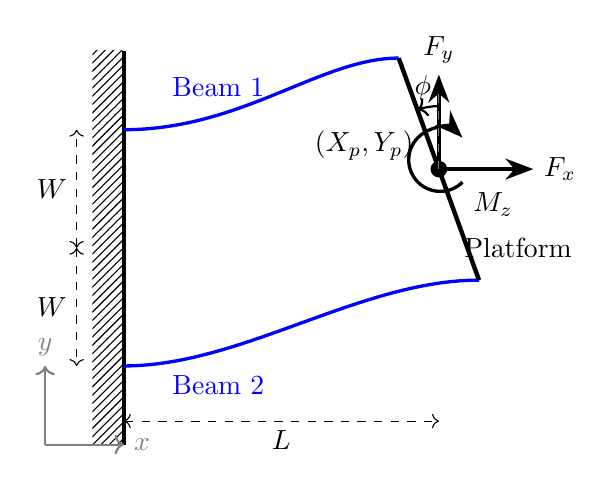
\begin{tikzpicture}
    % Ground
    \fill[pattern=north east lines] (-0.4,-2.5) rectangle (0,2.5);
    \draw[very thick] (0,-2.5) -- (0,2.5);
    
    % Upper beam (S-shape curve) - endpoint (3.49, 2.41) for phi=20 deg
    \draw[very thick, blue] (0,1.5) .. controls (1.5,1.5) and (2.5,2.41) .. (3.49,2.41);
    \node[above, blue] at (1.2,1.8) {Beam 1};
    
    % Lower beam (S-shape curve) - endpoint (4.51, -0.41) for phi=20 deg
    \draw[very thick, blue] (0,-1.5) .. controls (1.5,-1.5) and (3.0,-0.41) .. (4.51,-0.41);
    \node[below, blue] at (1.2,-1.5) {Beam 2};
    
    % Platform (Rotated by 20 degrees CCW)
    \draw[ultra thick, black] (4.51,-0.41) -- (3.49,2.41);
    \node[right, black] at (4.2,0) {Platform};
    
    % Platform center
    \fill (4,1) circle (3pt);
    \node[left] at (3.8,1.3) {$(X_p, Y_p)$};
    
    % External forces
    \draw[-{Stealth[scale=1.2]}, very thick, black] (4,1) -- (5.2,1) node[right] {$F_x$};
    \draw[-{Stealth[scale=1.2]}, very thick, black] (4,1) -- (4,2.2) node[above] {$F_y$};
    \draw[{Stealth[scale=1.2]}-, very thick, black] (4.3,1.4) arc (45:315:0.4) node[below right] {$M_z$};
    
    % Dimensions
    \draw[<->, dashed] (-0.6,0) -- (-0.6,1.5) node[midway, left] {$W$};
    \draw[<->, dashed] (-0.6,0) -- (-0.6,-1.5) node[midway, left] {$W$};
    \draw[<->, dashed] (0,-2.2) -- (4,-2.2) node[midway, below] {$L$};
    
    % Angle phi (CCW positive) - drawn at center for more amplification
    \draw[dashed, gray] (4,1) -- (4,2.0); % Vertical reference
    \draw[->, thick] (4,1.8) arc (90:110:0.8) node[above, xshift=2pt] {$\phi$};
    
    % Coordinate system
    \draw[->, thick, gray] (-1,-2.5) -- (0,-2.5) node[right] {$x$};
    \draw[->, thick, gray] (-1,-2.5) -- (-1,-1.5) node[above] {$y$};
\end{tikzpicture}%
}
\caption{Parallelogram flexure mechanism under external loading}
\label{fig:parallelogram}
\end{figure}

\subsection{Kinematic Constraint and Force Equilibrium Equations}
An external load $(F_x, F_y, M_z)$ is applied at the platform center $(X_p, Y_p)$. The static equilibrium of the platform, illustrated in Fig.~\ref{fig:platform_fbd}, requires that the horizontal, vertical, and moment reactions from both beams balance the applied external loads. These dimensional relations are subsequently mapped to a dimensionless form to facilitate numerical implementation.


\begin{figure}[ht]
\centering
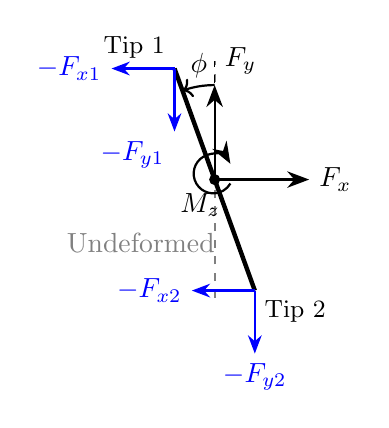
\begin{tikzpicture}[scale=1.0]
    % Undeformed Platform (dashed gray)
    \draw[thick, gray, dashed] (0,-1.5) -- (0,1.5);
    \node[right, gray] at (-2,-0.8) {Undeformed};
    
    % Deformed Platform Line (rotated 20 deg CCW)
    % phi = 20 deg. Tip 1 (Top): (-0.51, 1.41), Tip 2 (Bottom): (0.51, -1.41)
    \coordinate (Tip1) at (-0.51, 1.41);
    \coordinate (Tip2) at (0.51, -1.41);
    
    % Draw Platform
    \draw[ultra thick, black] (Tip2) -- (Tip1);
    \fill (0,0) circle (2pt); % Center
    
    % Label phi
    \draw[dashed] (0,0.8) -- (0,1.5); % Vertical reference
    \draw[->, thick, black] (0,1.2) arc (90:110:1.2);
    \node at (-0.2, 1.45) {$\phi$};
    
    % External forces at center
    \draw[-{Stealth[scale=1.2]}, thick, black] (0,0) -- (1.2,0) node[right] {$F_x$};
    \draw[-{Stealth[scale=1.2]}, thick, black] (0,0) -- (0,1.2) node[above right] {$F_y$};
    \draw[{Stealth[scale=1.2]}-, thick, black] (0.2,0.2) arc (30:330:0.25) node[below left] {$M_z$};
    
    % Tip 1 reactions
    \draw[-{Stealth}, thick, blue] (Tip1) -- ++(-0.8,0) node[left] {$-F_{x1}$};
    \draw[-{Stealth}, thick, blue] (Tip1) -- ++(0,-0.8) node[below left] {$-F_{y1}$};
    \node[above left] at (Tip1) {\small Tip 1};
    
    % Tip 2 reactions
    \draw[-{Stealth}, thick, blue] (Tip2) -- ++(-0.8,0) node[left] {$-F_{x2}$};
    \draw[-{Stealth}, thick, blue] (Tip2) -- ++(0,-0.8) node[below] {$-F_{y2}$};
    \node[below right] at (Tip2) {\small Tip 2};
\end{tikzpicture}
\caption{Free body diagram of the platform ($\phi > 0$)}
\label{fig:platform_fbd}
\end{figure}


\begin{table}[ht]
\centering
\caption{Normalized parameters for the parallelogram mechanism}
\label{tab:para_normalization}
\begin{tabular}{@{}ccc@{}}
\toprule
\textbf{Parameter} & \textbf{Definition} & \textbf{Description} \\
\midrule
$w$ & $W/L$ & Normalized half beam separation \\
$\alpha_{xi}$ & $F_{xi} L^2 / EI$ & Norm. horizontal reaction on beam $i$ \\
$\alpha_{yi}$ & $F_{yi} L^2 / EI$ & Norm. vertical reaction on beam $i$ \\
$\beta_i$ & $M_{zi} L / EI$ & Norm. moment on beam $i$ \\
$\alpha_x$ & $F_x L^2 / EI$ & Norm. external horizontal force \\
$\alpha_y$ & $F_y L^2 / EI$ & Norm. external vertical force \\
$\beta$ & $M_z L / EI$ & Norm. external moment \\
$u_x$ & $U_x/L$ & Norm. horizontal displacement \\
$u_y$ & $U_y/L$ & Norm. vertical displacement \\
$\phi$ & $-$ & platform rotation \\
\bottomrule
\end{tabular}
\end{table}

These static conditions are generalized using the normalized parameters defined in Table~\ref{tab:para_normalization}. The motion of the platform, characterized by a rotation $\phi$, imposes displacement and angle compatibility constraints at each beam tip. Together with the force and moment equilibrium, these relations constitute the full system of governing equations summarized in Table~\ref{tab:constraints}. The state is found by solving the coupled constraint equations (Table~\ref{tab:constraints}) iteratively using a Newton-Raphson scheme where each residual evaluation requires solving two beam BVPs.

\begin{table*}[t]
\centering
\caption{Summary of Equations for the Parallelogram Mechanism}
\label{tab:constraints}
\begin{tabular}{lll}
\toprule
\textbf{Category} & \textbf{Component} & \textbf{Equation} \\
\midrule
\textbf{Beam Physics} & Governing ODE & $\theta_i'' = \alpha_{xi} \sin\theta_i - \alpha_{yi} \cos\theta_i$ \\
(for $i=1, 2$) & Kinematics & $\xbar_i' = \cos\theta_i, \quad \ybar_i' = \sin\theta_i$ \\
& Fixed BCs & $\xbar_i(0)=0, \ybar_i(0)=0, \theta_i(0)=0$ \\
& Tip Reaction & $\theta_i'(1) = \beta_i$ \\
\midrule
\textbf{Platform} & Rotation & $\theta_1(1) = \phi, \quad \theta_2(1) = \phi$ \\
\textbf{Kinematics} & $x$-Compatibility & $\xbar_1(1) - \xbar_2(1) = -2w\sin\phi$ \\
& $y$-Compatibility & $\ybar_1(1) - \ybar_2(1) = 2w(\cos\phi - 1)$ \\
\midrule
\textbf{Mechanism} & Horiz. Equil. & $\alpha_{x1} + \alpha_{x2} = \alpha_x$ \\
\textbf{Statics} & Vert. Equil. & $\alpha_{y1} + \alpha_{y2} = \alpha_y$ \\
& Moment Equil. & $\beta_1 + \beta_2 - w\cos\phi \Delta\alpha_x - w\sin\phi \Delta\alpha_y = \beta$ \\
\bottomrule
\end{tabular}
\end{table*}

The complete system involves six unknowns $(\alpha_{x1}, \alpha_{y1}, \beta_1, \alpha_{x2}, \alpha_{y2}, \beta_2)$ and the platform rotation $\phi$, subject to the constraint equations summarized in Table~\ref{tab:constraints}.

\subsection{Hierarchical Modeling Stack}
To solve this problem, we develop a multi-fidelity modeling stack ranging from simple analytical models to high-fidelity FEA simulations. These modeling levels are summarized in Table~\ref{tab:modeling_stack}.

\begin{table}[ht]
\centering
\caption{The eight-level hierarchical modeling stack for the parallelogram mechanism}
\label{tab:modeling_stack}
\begin{tabular}{lll}
\toprule
\textbf{Model} & \textbf{Characteristic / Formulation} & \textbf{Section} \\
\midrule
Linear Theory & Small-angle, no coupling & Sec.~\ref{sec:linear} \\
BCM \cite{awtar2007characteristics} & Polynomial expansion, load-stiffening & Sec.~\ref{sec:bcm} \\
Guided BVP & Single beam surfing, no $\phi$ & Sec.~\ref{sec:guided} \\
Euler BVP & Full coupled nonlinear ODEs & Sec.~\ref{sec:euler} \\
PRB (Std.) & Rigid link approximation ($\gamma \approx 0.85$) & Sec.~\ref{sec:prbm} \\
PRB (Opt.) & Optimized link radius ($\gamma = 0.90$) & Sec.~\ref{sec:prbm} \\
FEA (2D) & Nonlinear beam elements (CalculiX) & Sec.~\ref{sec:fea} \\
FEA (3D) & Nonlinear solid elements (CalculiX) & Sec.~\ref{sec:fea} \\
\bottomrule
\end{tabular}
\end{table}

In the following, we will discuss each modeling level in detail.

\subsection{Linear Theory}
\label{sec:linear}
The simplest model assumes small-angle approximations ($\cos\theta \approx 1, \sin\theta \approx \theta$) and neglects the axial-transverse coupling. For the parallelogram mechanism consisting of two identical beams, the stiffness is doubled compared to a single guided beam ($12EI/L^3$), resulting in an equivalent stiffness of $24EI/L^3$. The resulting normalized displacements are:
\begin{equation}
u_y = \frac{\alpha_y}{24}, \quad u_x = 0, \quad \phi = 0 
\end{equation}
The axial shortening $u_x$ and parasitic rotation $\phi$ are identically zero in this first-order baseline. This model is implemented in \texttt{linear\_solver.py} using the \texttt{solve\_parallelogram} function and is valid only for very small deflections ($\alpha_y \ll 1$).

\subsection{Beam Constraint Model (BCM)}
\label{sec:bcm}
The BCM framework \cite{awtar2007characteristics}, utilizes polynomial expansions to approximate the transcendental beam functions. A key simplification in this approach is the assumption that the beam slope $dy/dx$ remains small (typically less than 10\%, or $\approx 0.1$). This allows the exact curvature expression $\kappa = \frac{d^2y/dx^2}{[1 + (dy/dx)^2]^{3/2}}$ to be simplified to the linear form $\kappa \approx d^2y/dx^2$. Despite this simplification, the model rigorously captures the nonlinear elastokinematic shortening and load-stiffening effects through axial-load dependent coefficients: $a(\alpha_x) = 12 + 1.2 \alpha_x - \frac{1}{700} \alpha_x^2$, $b(\alpha_x) = 4 + \frac{2}{15} \alpha_x - \frac{11}{6300} \alpha_x^2$, and $c(\alpha_x) = -6 - 0.1 \alpha_x + \frac{1}{1400} \alpha_x^2$.

For a symmetric parallelogram mechanism, the closed-form response is:
\begin{align}
u_y &= \frac{\alpha_y}{24 + 1.2 \alpha_x} \label{eq:bcm_uy} \\
u_x &= \alpha_x \left( \frac{t^2}{24} \right) - 0.6 u_y^2 + \frac{u_y^2 \alpha_x}{1400} \label{eq:bcm_ux} \\
\phi &= \frac{0.5}{w^2} \left[ \left( \frac{t^2}{12} + \frac{u_y^2}{700} \right) \left( \beta + u_y (12 + 0.1 \alpha_x) \right) \right] \label{eq:bcm_phi}
\end{align}
where $t$ is the normalized beam thickness. This model is implemented in \texttt{bcm\_parallelogram.py} and provides a highly efficient closed-form alternative for intermediate deflections.

\subsection{Solve for a Single Guided Beam}
\label{sec:guided}
This model serves as a high-fidelity surrogate that solves the exact nonlinear beam equations presented in Section~\ref{sec:beam_equations} for a single beam under a guided tip constraint ($\theta(1)=0$). It assumes that both beams in the mechanism are identical and undergo synchronized deformation, thereby neglecting the platform-level parasitic rotation ($\phi = 0$). In this simplified implementation, each beam carries exactly half of the normalized loads ($\alpha_x/2$ and $\alpha_y/2$), and any externally applied moment $\beta$ is ignored as it is balanced by the guided constraint reaction. While it does not capture the coupling that leads to stage rotation, it provides a rigorous solution for large deflections using a numerical Boundary Value Problem (BVP) solver. This model is implemented in \texttt{guided\_beam\_solver.py}.



\subsection{Solve for Two Coupled Euler Beams}
\label{sec:euler}
The most rigorous analytical approach involves solving the full set of coupled nonlinear equations derived in Section 2 and summarized in Table~\ref{tab:constraints}. Unlike the single-beam surrogate, this model treats each beam in the parallelogram individually, solving for their respective internal end loads $(\alpha_{x1}, \alpha_{y1}, \beta_1)$ and $(\alpha_{x2}, \alpha_{y2}, \beta_2)$. This differentiation is critical because the mechanism's geometry and the externally applied loads induce different axial forces in each beam—typically placing one beam in tension while the other is in compression. 

By capturing this asymmetry and the resulting differential beam shortening, the model successfully predicts the platform's parasitic rotation angle $\phi$. The system of equations is solved using a nested iterative approach: an outer root-finding loop handles the 6 platform constraints, while an inner boundary value problem (BVP) solver based on a 4th-order collocation method (implemented via \texttt{scipy.integrate.solve\_bvp}) computes the individual beam shapes for a given set of end loads. This complete multi-beam solution is implemented in \texttt{parallelogram\_solver.py} and serves as the ultimate analytical benchmark for our study.

The system is solved using the following iterative scheme:
\begin{enumerate}
    \item \textbf{Initialize:} Guess initial values for the 6 internal platform loads $[\alpha_{x1}, \alpha_{y1}, \beta_1, \alpha_{x2}, \alpha_{y2}, \beta_2]$.
    \item \textbf{Solve Beams:} For each beam, solve the normalized ODE BVP (Eq.~\eqref{eq:normalized_ode}) for current load guesses. A cubic polynomial guess matching fixed-guided behavior is used to initialize the collocation solver.
    \item \textbf{Compute Residuals:} Evaluate the 6 platform compatibility and equilibrium constraints (Table~\ref{tab:constraints}).
    \item \textbf{Update:} Use a Jacobian-based numerical root-solver (e.g., \texttt{hybr} or \texttt{lm}) to update guesses until residuals vanish below $\epsilon = 10^{-6}$.
    \item \textbf{Result:} Extract platform displacement ($\bar{X}_p, \bar{Y}_p$) and rotation $\phi$.
\end{enumerate}


\begin{figure}[ht]
\centering
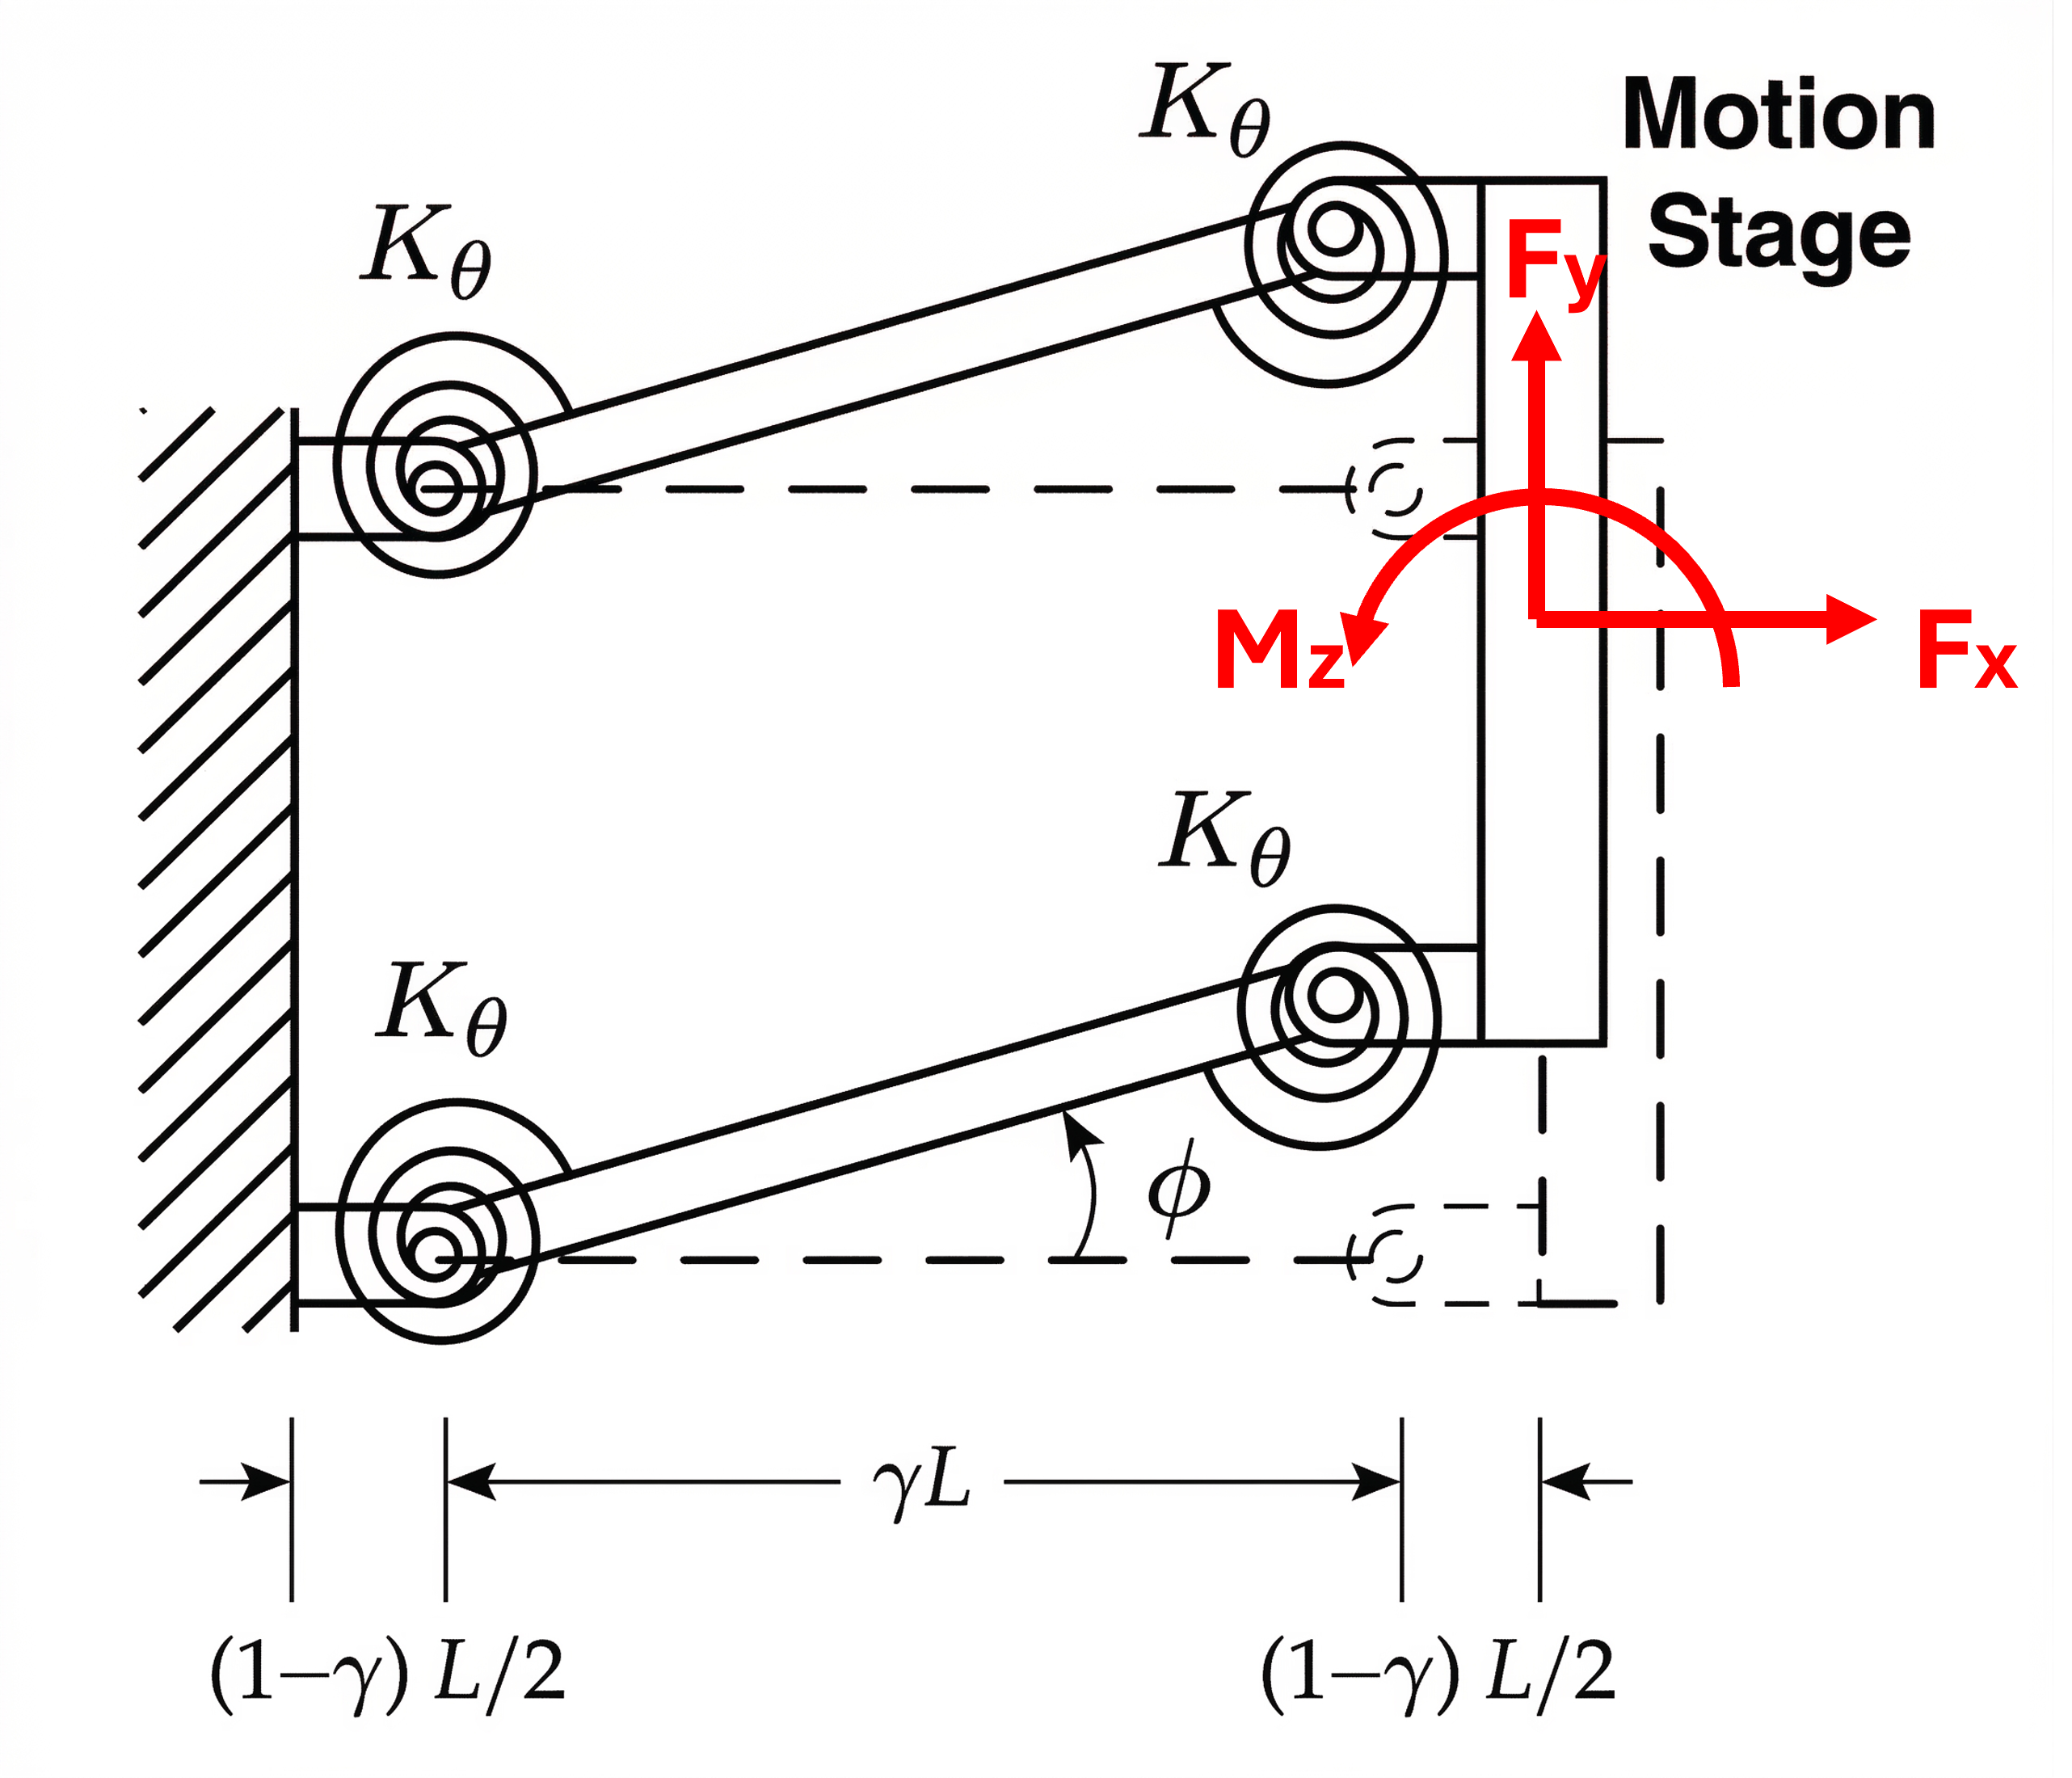
\includegraphics[width=0.75\columnwidth]{images/PRBM_Label.png}
\caption{PRB schematic of the parallelogram flexure. Each beam is modeled as a serial chain of 2R with rigid segments $(1-\gamma)L/2$ and pseudo-links $\gamma L$. Torsional springs at the pivots have stiffness $K = 2 \gamma K_\Theta EI/L$. External loads are applied at the stage center $(X_p, Y_p)$.}
\label{fig:prb_schematic}
\end{figure}

\subsection{Pseudo-Rigid-Body Model (PRBM)}
\label{sec:prbm}
The PRBM approximates large-deflection flexures by replacing flexible segments with rigid pseudo-links and torsional springs \cite{Howell1994, Howell1995}. For the parallelogram flexure, the entire mechanism is modeled as a 4-bar linkage (Fig.~\ref{fig:prb_schematic}), where each beam is represented by a rigid link of characteristic length $\gamma L$ and two horizontal segments of length $(1-\gamma)L/2$. This simplifies the S-shaped deformation into a pure rotary motion of the platform. While higher-order models like Su's 3R model \cite{Su2009PRB3R} provide superior accuracy for single cantilever beams, the 1R model remains the computational baseline for mechanism-level synthesis. The kinematic relations are defined as:
\begin{equation}
u_y = \gamma \sin \Theta, \quad u_x = \gamma (\cos \Theta - 1)
\end{equation}
where $\Theta$ is the pseudo-rigid-body angle. Each pivot is equipped with a torsional spring of stiffness $K =2 \gamma K_\Theta \frac{EI}{L}$. For the symmetric dual-beam mechanism, the static equilibrium yields a nonlinear transcendental equation for $\Theta$:
\begin{equation}
K \Theta = \frac{F_y}{2}  \frac{\gamma L}{2} \cos \Theta
\label{eq:prb_equilibrium}
\end{equation}
where the factors of 2 account for the parallel combination of two beams, with each beam effectively acting as a 1R cantilever under half the total load ($\alpha_y/2$).

The coefficients $\gamma$ and $K_\Theta$ are critical for model accuracy across different loading regimes. While standard textbook values (e.g., $\gamma=0.8517$ for fixed-guided beam with a vertical end force) work well for moderate deflections, they often fail to capture the behavior under high axial prestress or near-buckling conditions. Consequently, an optimized set of parameters was obtained by minimizing the Root-Mean-Square Error (RMSE) of the transverse deflection $u_y$ relative to the nonlinear Euler BVP ground truth over a sweep of $\alpha_y \in [-15, 15]$ (see \texttt{gamma\_study.py}). As shown in Table~\ref{tab:modeling_stack}, the optimized model utilizes a higher $\gamma$ factor (0.900), which better approximates the "softening" effect and shape changes caused by internal buckling forces. This optimization improves the prediction of vertical stiffness and kinematic shortening $u_x$ with $K_\Theta$ refined to 2.5. The model is implemented in \texttt{prb\_parallelogram.py} using a numerical solver for Eq.~\eqref{eq:prb_equilibrium}.


\subsection{Finite Element Analysis (FEA)}
\label{sec:fea}
The final two levels of the hierarchy utilize numerical discretization to provide high-fidelity verification and ground-truth validation. Both 2D and 3D FEA models are implemented using the open-source solver \texttt{CalculiX} with the geometrically nonlinear (NLGEOM) solver option enabled. Since these numerical solvers operate on absolute dimensions, the benchmark mechanism is modeled using the geometric and material properties summarized in Table~\ref{tab:model_params} (structural steel). The external moment $\beta$ is applied via a horizontal force couple at $y = \pm 10\text{ mm}$ for 3D and $y = \pm 50\text{ mm}$ for 2D relative to the stage center. The setup parameters for both models are summarized in Table~\ref{tab:fea_setup}.

\begin{table}[ht]
\centering
\caption{Benchmark Model Parameters}
\label{tab:model_params}
\begin{tabular}{lc|lc}
\toprule
\textbf{Param.} & \textbf{Value} & \textbf{Param.} & \textbf{Value} \\
\midrule
$L$ & 250.0 mm & $E_{beam}$ & 210.0 GPa \\
$W$ & 75.0 mm & $E_{stage}$ & 5000.0 GPa \\
$H$ & 50.0 mm & $\nu$ & 0.3 \\
$T$ & 5.0 mm & $L_{m}$ & 50.0 mm \\
$I_{beam}$ & $520.83 \text{ mm}^4$ & & \\
\bottomrule
\end{tabular}
\end{table}

\begin{table}[ht]
\centering
\caption{FEA Simulation Setup Parameters}
\label{tab:fea_setup}
\begin{tabular}{lcc}
\toprule
\textbf{Parameter} & \textbf{2D Model} & \textbf{3D Model} \\
\midrule
Element Type & B32 (Quadratic Beam) & C3D10 (Quadratic Tet) \\
Mesh Size & $L_c = 6.5$~mm & 10 mm (Global) \\
Mesh Order & 2nd & 2nd \\
Nonlinearity & NLGEOM & NLGEOM \\
Platform &  Quasi-Rigid & Quasi-Rigid \\
\bottomrule
\end{tabular}
\end{table}

The 2D FEA utilizes quadratic beam elements with a characteristic mesh length of $6.5$~mm ($L_c = 6.5$~mm) for both the flexures and the platform stage. The motion stage is modeled as a rigid coupling between the beam tips, accurately representing the $2W$ linkage constraint. This level serves as a verification for the Euler-Bernoulli assumptions in local coordinates without Section 2's shooting method complexity.

The 3D ground truth model uses solid elements to capture stress-stiffening, out-of-plane effects, and the localized compliance of the base/stage interfaces. A mesh convergence study demonstrated that a global mesh size of 10 mm is sufficient for capturing the nonlinear displacement field, yielding results within $1.1\%$ of a refined 5 mm mesh while significantly reducing computational time. The monolithic geometry includes integrated base blocks and the stage, allowing for a complete assessment of the analytical models against a full-scale solid mechanic's simulation. The implementation scripts for running these FEA solvers are publicly available in our GitHub repository.


\section{Data Generation and Runtime Comparison}
\subsection{Data Generation}
A benchmark loading grid was established to verify the reduced-order models. The simulation sweep consists of 1,517 distinct load cases covering the normalized ranges summarized in Table~\ref{tab:load_sweep}. Both 2D beam and 3D solid FEA solvers were executed across this entire grid to generate ground-truth displacement fields. 

To ensure complete coverage of the bilateral workspace, the simulation data were augmented using mirror symmetry about the $x$-axis. While the primary FEA sweep was computed for positive transverse loads ($\alpha_y \geq 0$), the negative range ($\alpha_y < 0$) was derived using the mapping $(\alpha_y, \alpha_x, \beta) \to (-\alpha_y, \alpha_x, -\beta)$, which corresponds to a response mapping of $(u_x, u_y, \phi) \to (u_x, -u_y, -\phi)$. This augmentation effectively doubles the dataset to 3,094 load points, covering the full symmetric range $\alpha_y \in [-20, 20]$.

\begin{table}[ht]
\centering
\caption{Normalized Load Sweep Grid Ranges}
\label{tab:load_sweep}
\begin{tabular}{ll}
\toprule
\textbf{Load } & \textbf{Discrete Values} \\
\midrule
$\alpha_y$ & $\{0, 0.5, 1, 2, \dots, 10, 12, \dots, 20\} \cup \text{Symmetric}$ \\
$\alpha_x$ & $\{-10, -5, -4, -3, -2, -1, 0, 1, 2, 3, 4, 5, 10\}$ \\
$\beta$ & $\{-3, -2, -1, 0, 1, 2, 3\}$ \\
\bottomrule
\end{tabular}
\end{table}

The 3D FEA data generation utilized parallel execution with 10 worker processes, completing the 1,547-case sweep in approximately 3 hours of wall-clock time (integrated solver time of 19.02 hours). In contrast, the 2D FEA sweep was executed on a single CPU core, requiring approximately 32.5 minutes (0.54 hours) to complete. The complete multi-fidelity dataset, including raw FEA outputs and pre-processed analytical results, is publicly available on the project's GitHub repository for further analysis and benchmarking.

\subsection{Computational Efficiency Comparison}
The performance of each modeling level is summarized in Table~\ref{tab:runtime_comparison}, using the 3D solid FEA as the baseline for computational speedup.
\begin{table}[ht]
\centering
\caption{Computational Performance and Speedup vs. 3D FEA}
\label{tab:runtime_comparison}
\begin{tabular}{lrcr}
\toprule
\textbf{Model} & \textbf{Success Rate} & \textbf{Mean $t$ / case (s)} & \textbf{Speedup} \\
\midrule
FEA 3D & 1547 / 1547 & 4.43E+01 & 1.00 \\
FEA 2D & 1547 / 1547 & 1.26E+00 & 35.14 \\
Euler BVP & 1425 / 1547 & 2.86E+00 & 15.46 \\
Guided Beam & 1547 / 1547 & 3.17E-03 & 1.40E+04 \\
PRB (Std/Opt) & 1547 / 1547 & $\sim$1.00E-04 & $\sim$4.50E+05 \\
BCM & 1547 / 1547 & 3.45E-06 & 1.28E+07 \\
Linear & 1547 / 1547 & 3.73E-07 & 1.18E+08 \\
\bottomrule
\end{tabular}
\end{table}

The efficiency analysis reveals a dramatic spread in computational cost across the stack. While high-fidelity 3D FEA requires tens of seconds per case, the closed-form BCM and Linear models achieve speedups of seven to eight orders of magnitude ($>10^7\times$). It is important to note that the Euler BVP model failed to converge in 122 cases (a 92\% success rate), primarily in regimes involving very large deflections or high compressive axial loads approaching buckling. This highlights the trade-off between the mathematical rigor of the S-shaped BVP solution and the robust numerical stability of FEA or the algebraic stability of BCM.

\subsection{Interactive Visualization and Benchmarking App}
To facilitate real-time exploration of the modeling hierarchy, we developed an interactive Python-based application (\texttt{compare\_models\_gui.py}). This tool allows users to manually adjust loading parameters $(\alpha_x, \alpha_y, \beta)$ and geometric dimensions (such as the normalized separation $w$) using sliders, providing immediate visual feedback on the resulting mechanism deformation. 

As shown in Fig.~\ref{fig:shape_comparison}, the app overlays the deformed shapes predicted by each model in the hierarchy. This visual comparison is particularly useful for identifying the limits of linearity and the onset of axial shortening ($u_x$). The interface also includes a live comparison table that reports the primary displacements $(u_x, u_y, \phi)$ and computes percentage errors relative to the high-fidelity 3D FEA benchmark. 

A notable feature is the integration of "live" solvers: while many results are retrieved from pre-computed sweeps for speed, the app can also invoke the FreeCAD-based FEA and Euler BVP solvers on-demand for arbitrary load cases. It is important to note that for the BCM level, the visualized beam shape is nominal (based on standard cubic interpolation) because the model's fundamental output is the platform's pose $(u_x, u_y, \phi)$ rather than the internal beam discretization. 

The development of this interactive tool and the underlying solver stack was significantly accelerated through the assistance of an AI coding agent (based on the Codex 5.4 model), which aided in the construction of the Matplotlib-based GUI and the orchestration of the cross-platform FEA scripts. The complete application, including all multi-fidelity solvers and benchmark datasets, is publicly available on the project's GitHub repository. This tool serves as a powerful benchmarking platform for validating low-fidelity models against rigorous numerical solutions across the entire workspace.

\begin{figure}[ht]
\centering
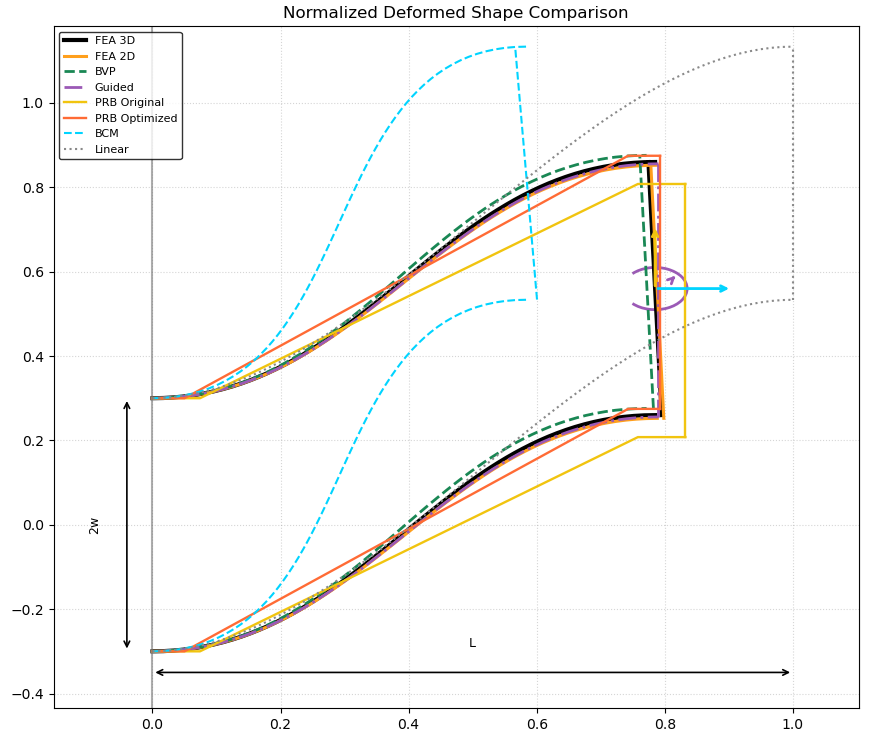
\includegraphics[width=1\columnwidth]{images/shape_all_model.png}
\caption{Screenshot of the interactive benchmarking app showing the normalized deformed shapes for multiple models. The plots shows the deformed shapes for $\alpha_x=0, \alpha_y=20, \beta=0$. Users can toggle visibility for specific models and monitor real-time error metrics as loading parameters are varied.}
\label{fig:shape_comparison}
\end{figure}

\begin{figure}[ht]
\centering
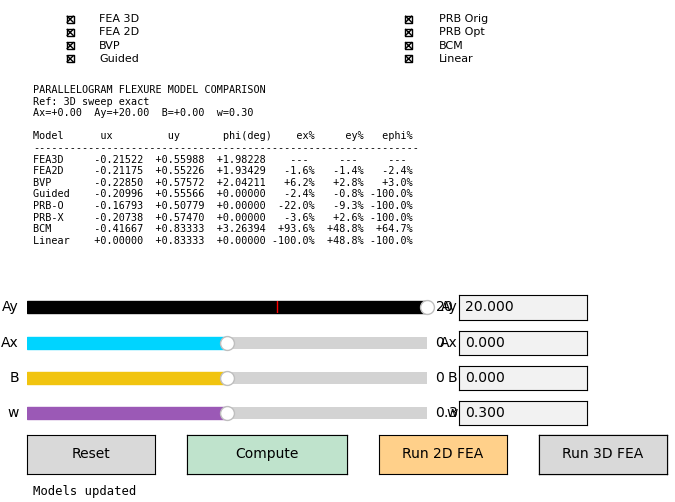
\includegraphics[width=1\columnwidth]{images/plot_app_interface.png}
\caption{User interface of the interactive benchmarking app. The control panel (bottom) includes sliders for loading and geometry, model visibility toggles, and buttons for live FEA triggering.}
\label{fig:app_interface}
\end{figure}

\section{Accuracy Assessment and Comparative Studies}
\label{sec:comparative_studies}
We conduct a comprehensive comparative study to evaluate the accuracy and efficiency of the eight-level modeling stack. 

\subsection{Case 1: \texorpdfstring{$\alpha_x = \beta = 0$}{alpha_x = beta = 0}}
The first case considers pure transverse loading ($\alpha_y$) in the absence of axial forces and external moments. This scenario isolates the primary stiffness and kinematic shortening effects. 

The primary stiffness response ($u_y$ vs. $\alpha_y$) is captured accurately by most models in the small deflection regime ($\alpha_y < 2$), with the BCM and Euler BVP models providing errors below 4\%. However, as the loading increases, the accuracy of the algebraic BCM model degrades; its relative error reaches approximately 8\% at $\alpha_y = 5$ and grows to nearly 50\% as $\alpha_y$ approaches 20. Specifically, the standard PRB model for $y$-deflection exhibits a larger error (15.51\%) in the small deflection regime, which notably reduces to 10.69\% at $\alpha_y = 20$, indicating that the model is effectively optimized for overall performance across a very large range of motion. The optimized PRB model consistently outperforms both the standard PRB and BCM across most of the force range. In contrast, the Euler BVP model and 2D FEA maintain high accuracy relative to the 3D solid ground truth, with errors around 3\% and 1.2\% respectively at the maximum load. 

The kinematic shortening effect ($u_x$ vs. $\alpha_y$) reveals a clear divergence in model fidelity. By definition, the Linear model fails to capture any axial shortening, resulting in a consistent 100\% relative error. In contrast, both the Euler BVP and 2D FEA models capture the parabolic shortening trend with high precision, maintaining errors within 7\% and 1.6\% respectively across the entire range. While the PRB models and the Guided Beam approximation perform well (with optimized PRB error reducing to 3.4\% at $\alpha_y = 20$), the algebraic BCM model exhibits significant performance degradation at higher loads. The BCM's relative error for $u_x$ starts at approximately 7.6\% in the small-deflection regime but grows to over 60\% as the loading approaches the workspace limits, underscoring its limitations in capturing second-order kinematic couplings at extreme deflections.

A critical result is observed in the prediction of parasitic rotation $\phi$. While the 3D FEA reveals a small but non-zero rotation reaching approximately $0.4^\circ$, the low-order models (Guided Beam, Linear, and PRB) assume zero rotation by definition, leading to 100\% relative error in this metric. The Euler BVP model, which accounts for the differential shortening between the two beams, predicts $\phi$ with increasing accuracy as the deflection grows, reaching a 3.3\% error at $\alpha_y = 20$. 2D FEA remains the most accurate non-reference model for $\phi$, with errors consistently around 2.2\%.

A comparison between the PRBM and BCM models highlights their relative advantages for parallelogram flexure modeling. The BCM is generally more accurate in the small-to-moderate loading range ($\alpha_y \in [0, 5]$); however, for larger deformations, the standard PRB model provides better scaling for the primary stiffness. Notably, the optimized PRB model outperforms the BCM in predicting both $u_y$ and $u_x$ across the entire loading range. It must be emphasized, however, that all PRB-based models are inherently limited by their simplified kinematics and cannot predict the parasitic rotation $\phi$.

\begin{figure}[ht!]
    \centering
    \begin{subfigure}[b]{\columnwidth}
        \centering
        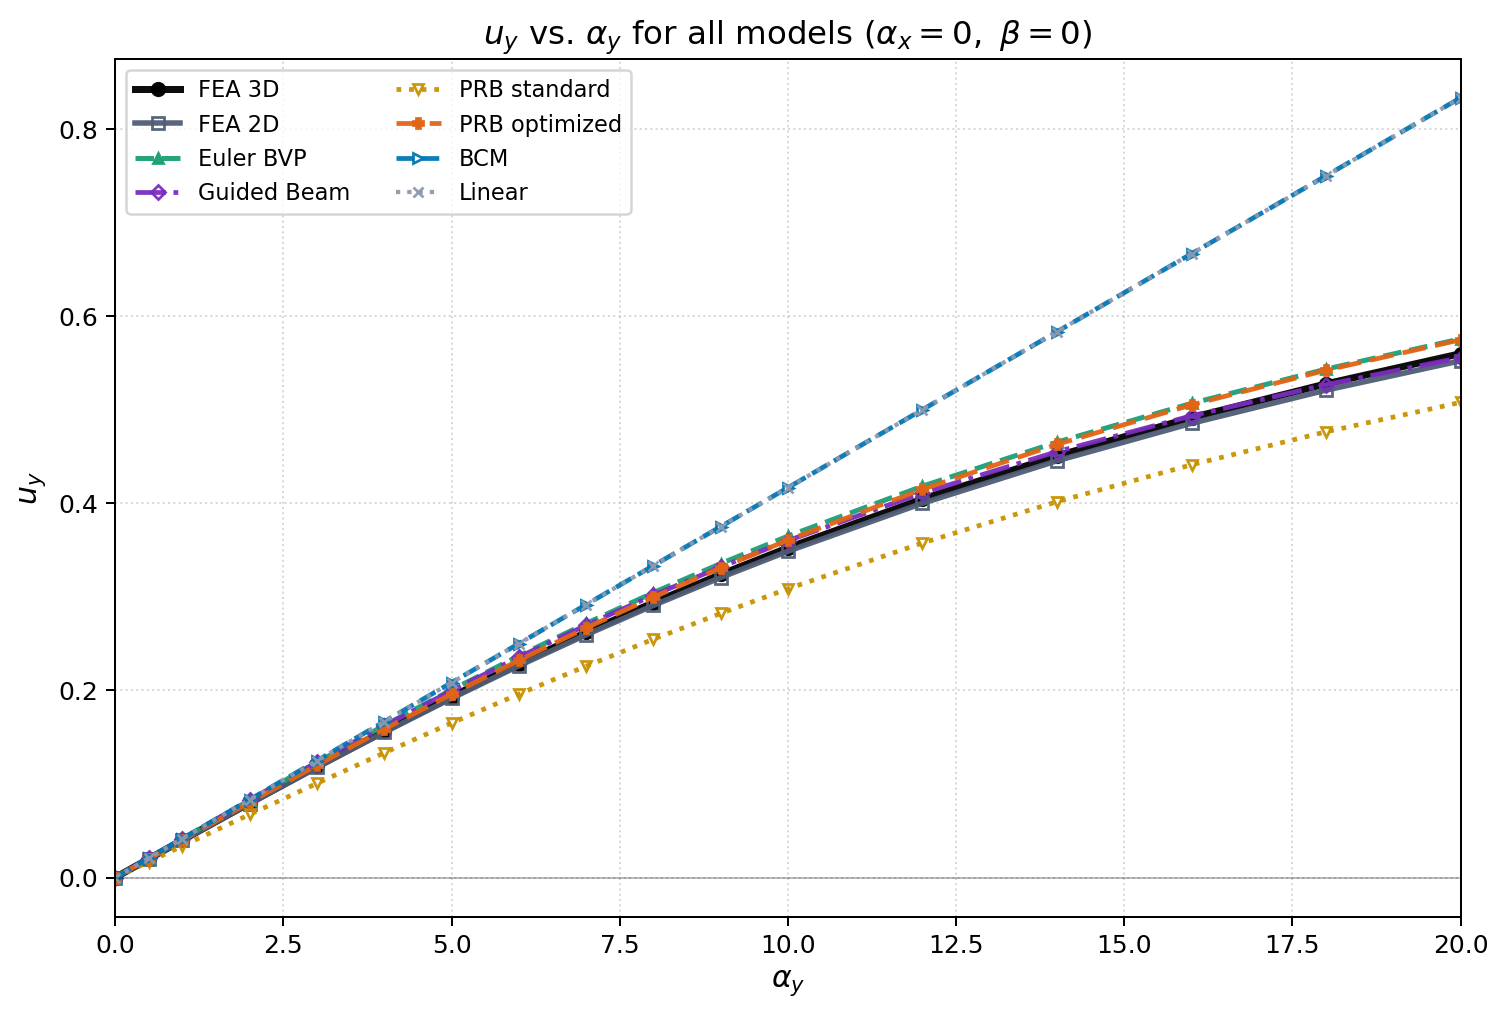
\includegraphics[width=0.95\columnwidth]{images/uy_vs_Ay_all_models_Ax0_B0.png}
        \caption{$u_y$ vs. $\alpha_y$}
    \end{subfigure}
    \vspace{0.3cm}
    \begin{subfigure}[b]{\columnwidth}
        \centering
        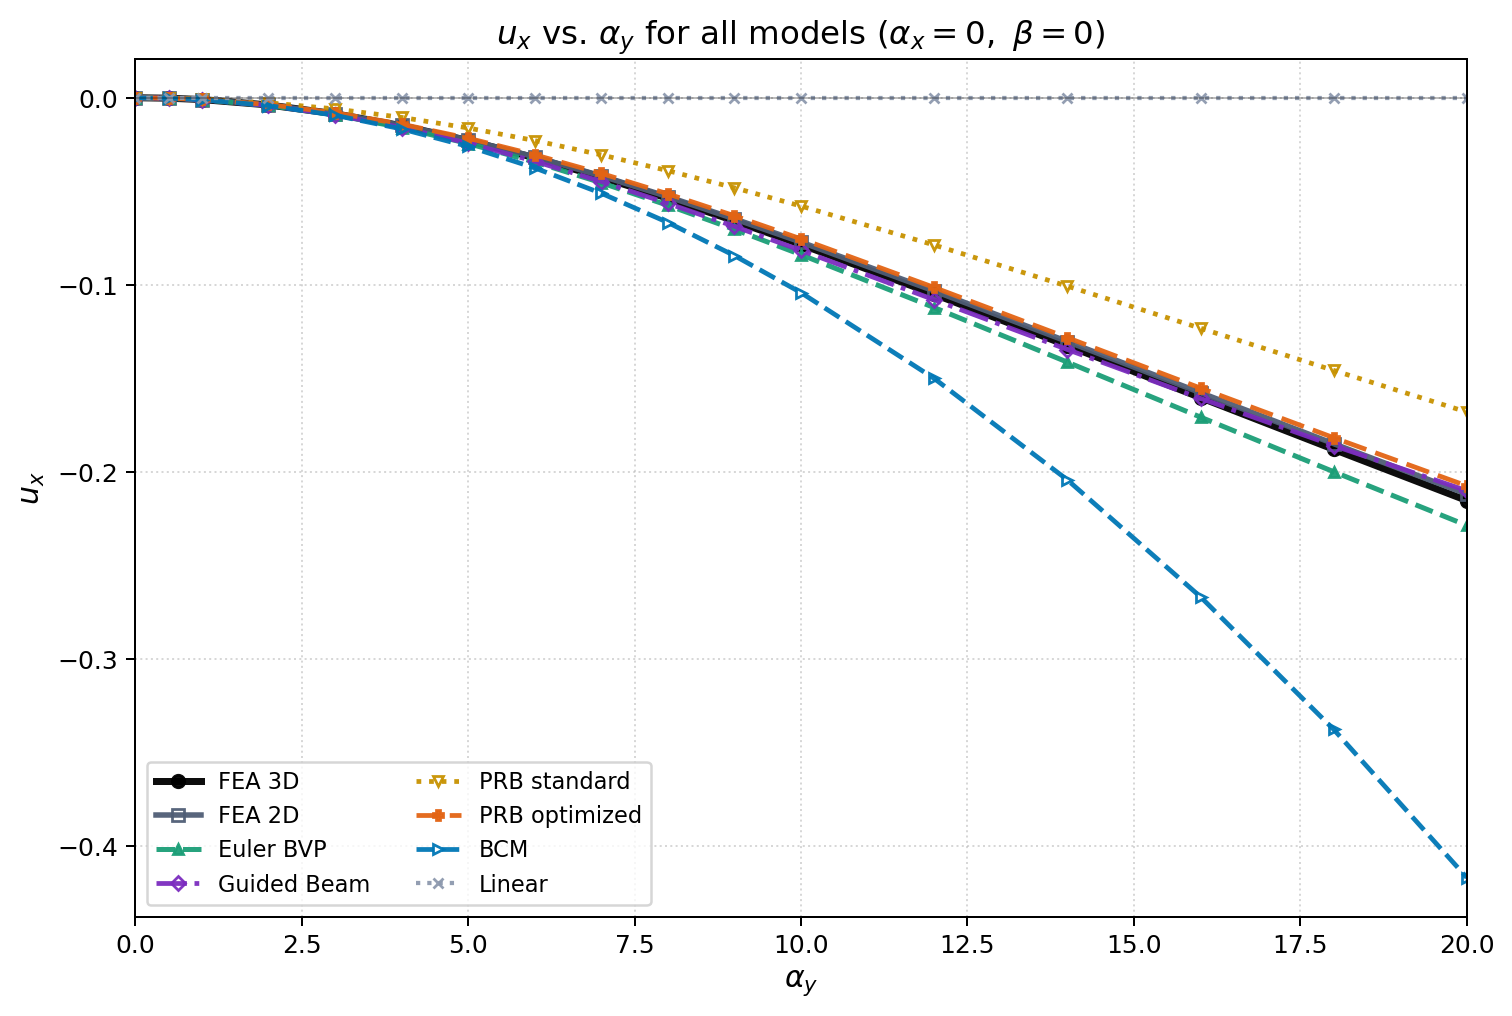
\includegraphics[width=0.95\columnwidth]{images/ux_vs_Ay_all_models_Ax0_B0.png}
        \caption{$u_x$ vs. $\alpha_y$}
    \end{subfigure}
    \vspace{0.3cm}
    \begin{subfigure}[b]{\columnwidth}
        \centering
        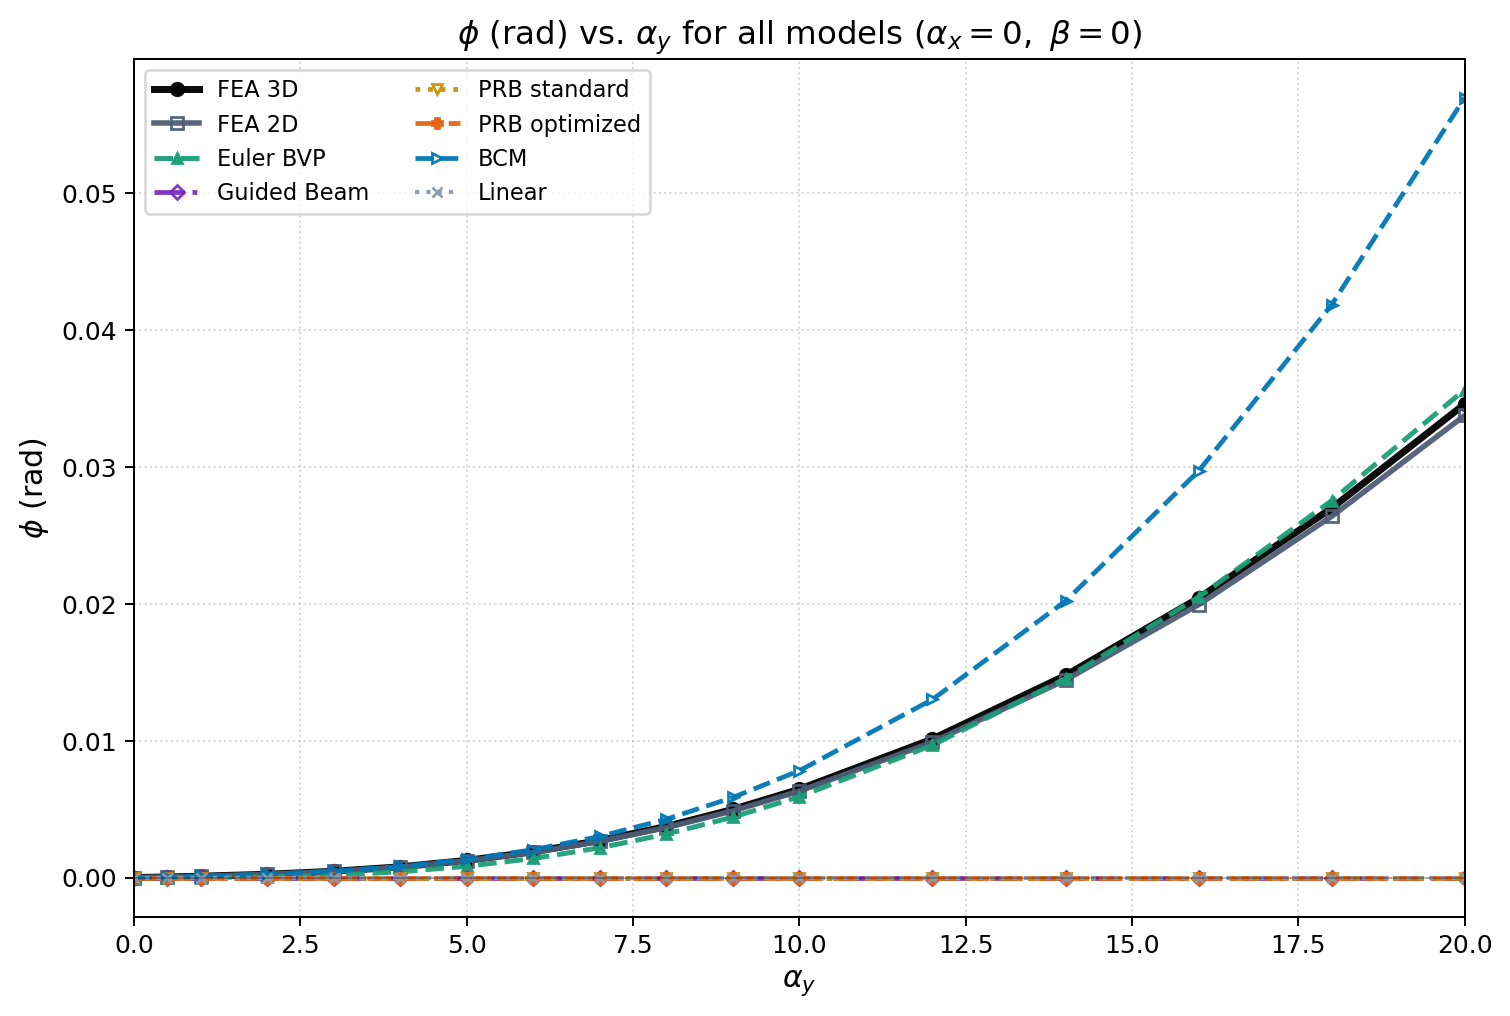
\includegraphics[width=0.95\columnwidth]{images/phi_vs_Ay_all_models_Ax0_B0.png}
        \caption{$\phi$ vs. $\alpha_y$}
    \end{subfigure}
    \caption{Mechanism response under pure transverse loading ($\alpha_x = \beta = 0$). The low-order models fail to capture the parasitic rotation $\phi$.}
    \label{fig:case1_accuracy}
\end{figure}

\begin{figure}[ht!]
    \centering
    \begin{subfigure}[b]{\columnwidth}
        \centering
        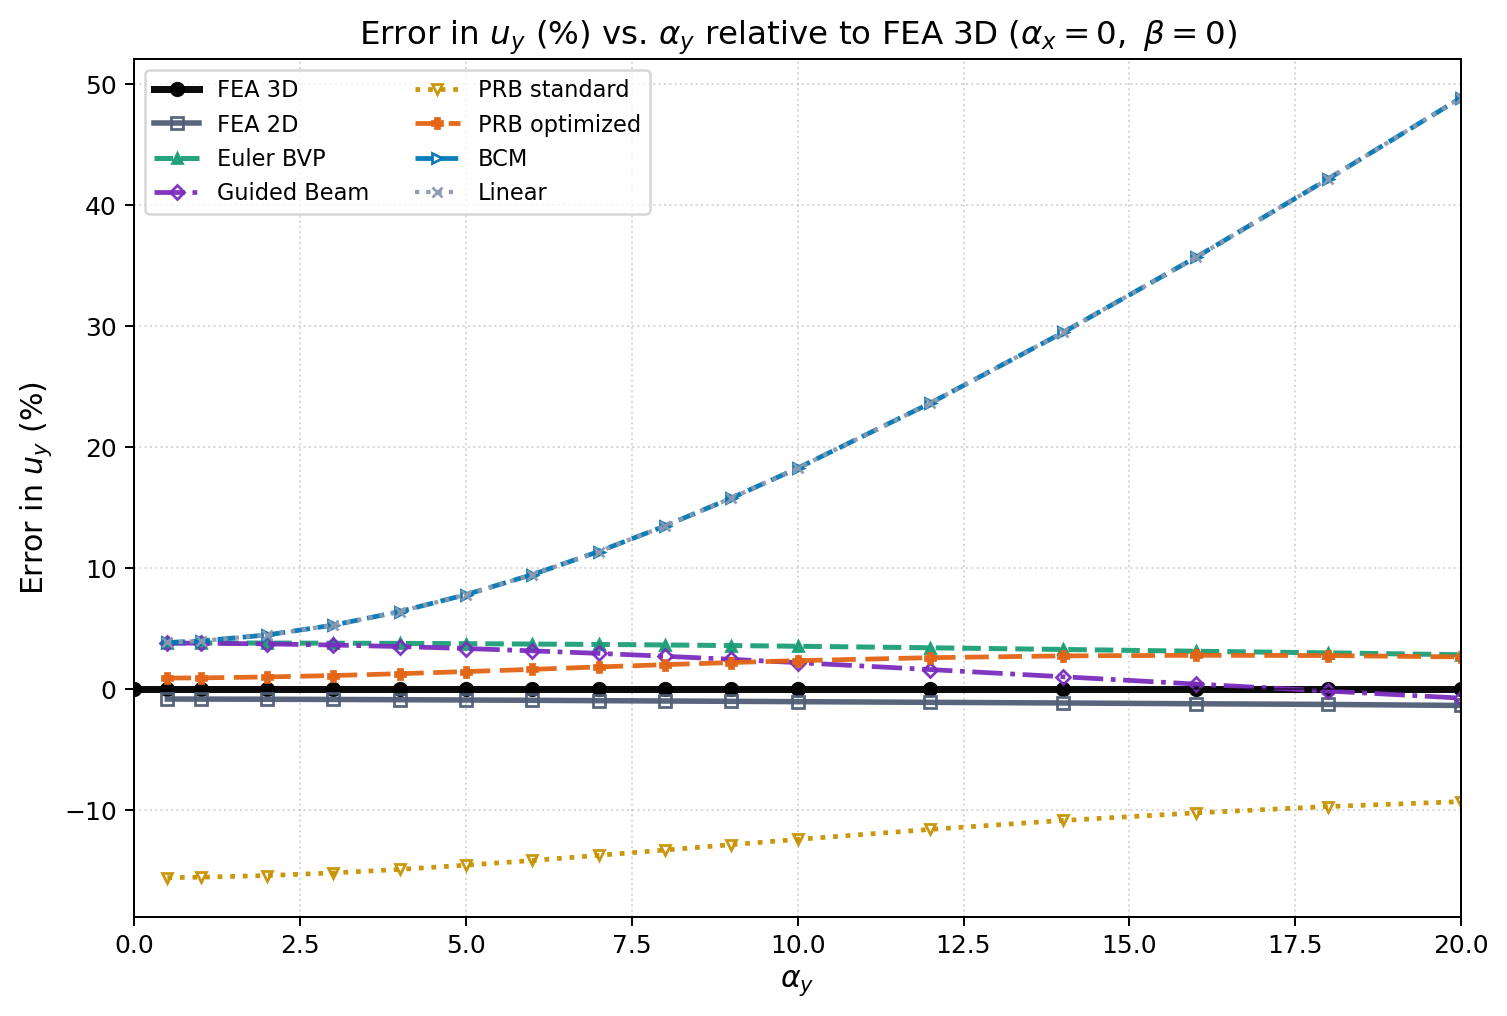
\includegraphics[width=0.95\columnwidth]{images/uy_error_pct_vs_Ay_all_models_Ax0_B0.png}
        \caption{Relative error in $u_y$}
    \end{subfigure}
    \vspace{0.3cm}
    \begin{subfigure}[b]{\columnwidth}
        \centering
        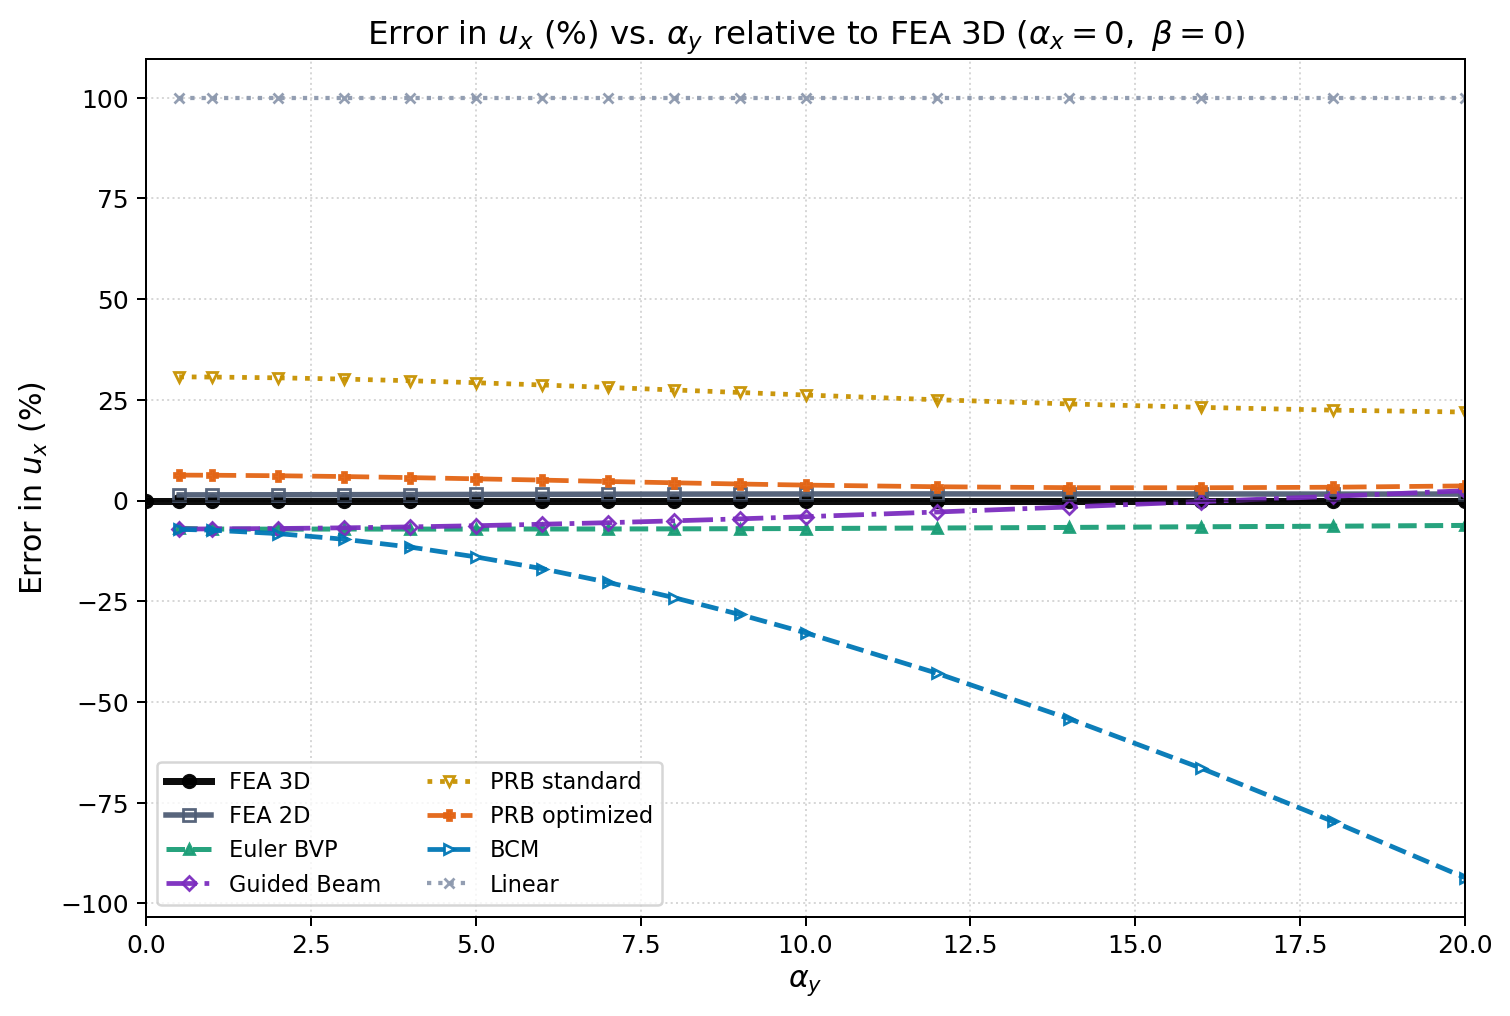
\includegraphics[width=0.95\columnwidth]{images/ux_error_pct_vs_Ay_all_models_Ax0_B0.png}
        \caption{Relative error in $u_x$}
    \end{subfigure}
    \vspace{0.3cm}
    \begin{subfigure}[b]{\columnwidth}
        \centering
        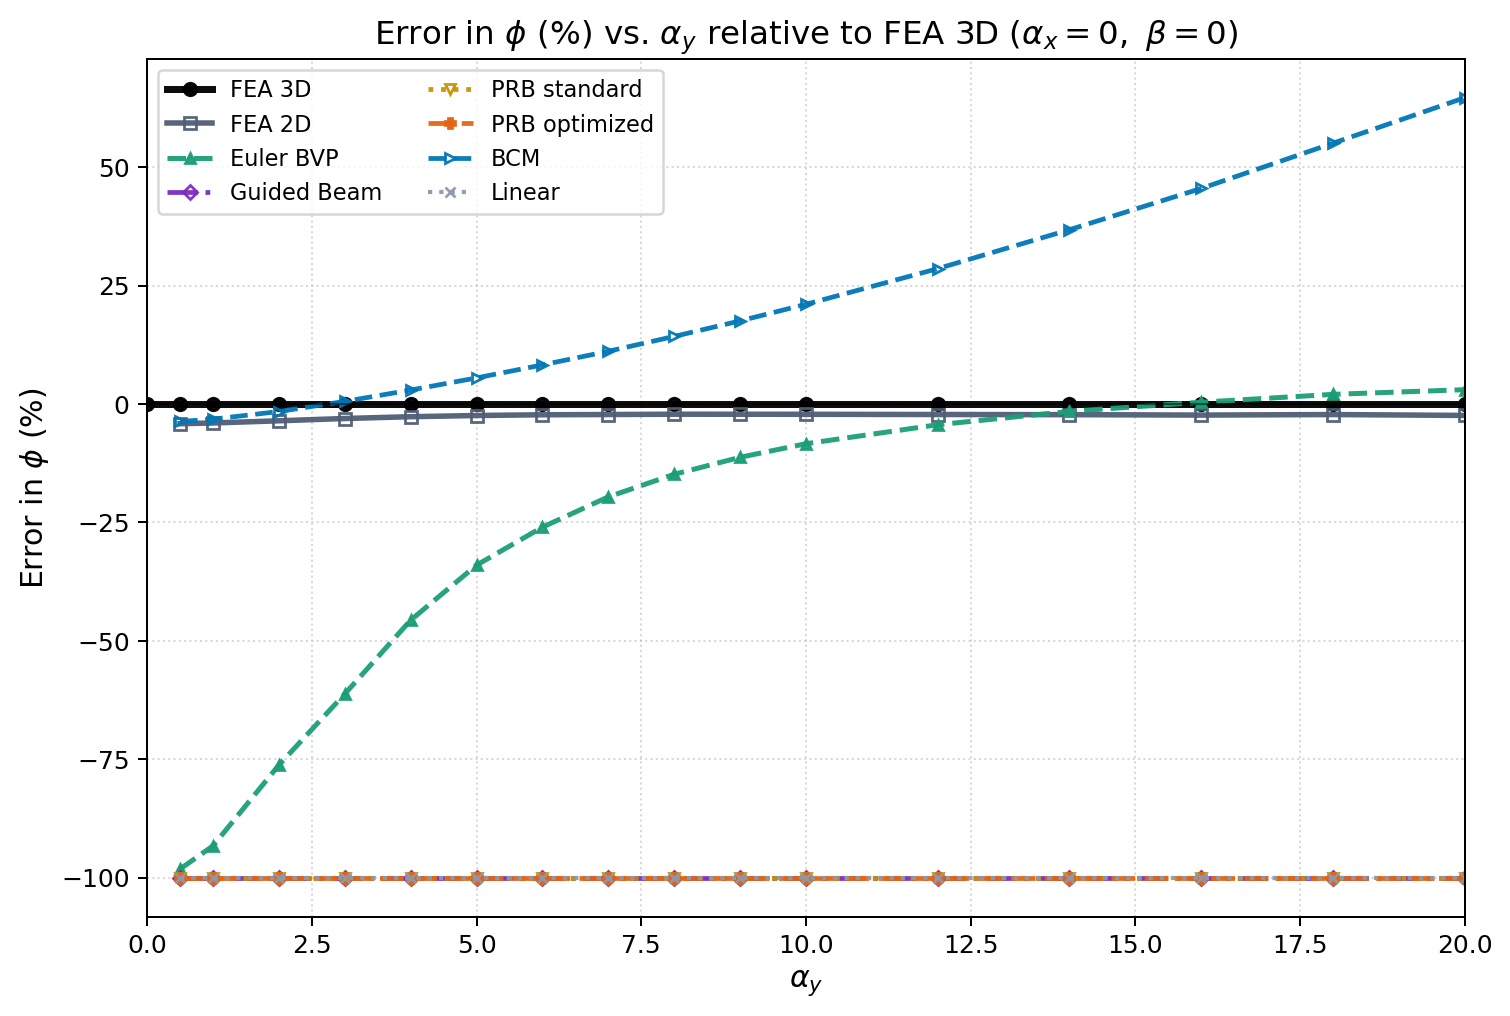
\includegraphics[width=0.95\columnwidth]{images/phi_error_pct_vs_Ay_all_models_Ax0_B0.png}
        \caption{Relative error in $\phi$}
    \end{subfigure}
    \caption{Relative error percentages for modeling levels under pure transverse loading ($\alpha_x = \beta = 0$) relative to the 3D FEA ground truth.}
    \label{fig:case1_errors}
\end{figure}

\subsection{Case 2: \texorpdfstring{$\alpha_x = -3, \beta = 0$}{alpha_x = -3, beta = 0}}
In Case 2, we introduce a significant compressive axial load ($\alpha_x = -3$), which approaches the critical buckling load of the flexure system. The primary transverse displacement $u_y$ (Fig.~\ref{fig:case2_accuracy}a) shows that most analytical models begin to diverge significantly from the 3D FEA ground truth even at moderate transverse loads ($\alpha_y > 5$). The BCM, while accurate for small deflections, exhibits a massive error growth---reaching 42.94\% at $\alpha_y = 20$---as it fails to capture the nonlinear interaction between the high transverse deflection and the near-buckling axial compression. In contrast, the optimized PRB model maintains a much lower error around 6.33\% in the high-load range, demonstrating its robustness in capturing the effective stiffness under prestressed conditions.

The kinematic shortening $u_x$ (Fig.~\ref{fig:case2_accuracy}b) is particularly sensitive to the compressive load. The standard PRB and BVP models show substantial errors (up to 38\% and 7.6\% respectively) when $\alpha_y$ is large, as the compressive force $\alpha_x$ amplifies the geometric non-linearity. The linear model, as expected, predicts zero $u_x$ and is completely invalid. Interestingly, the Guided Beam model performs exceptionally well for $u_x$ in this case (error $\sim$2.51\%), suggesting that its energy-based derivation captures the axial-transverse coupling quite effectively even under compressive stress, provided the transverse load is large enough to dominate the deformation shape.

The parasitic rotation $\phi$ (Fig.~\ref{fig:case2_accuracy}c) under compressive load reveals the limitations of simplified modeling levels. While the BCM remains the best analytical predictor for $\phi$ across much of the range (mean error $\sim$29\%), the absolute values of rotation are significantly influenced by the axial load. At low transverse loads ($\alpha_y < 2$), the errors for all models are extremely high ($>100$\% for beam-based models) due to the unstable nature of the "guided" state near the buckling threshold. These results highlight that for precision mechanisms operating under high axial compressive loads, relying on low-fidelity models can lead to catastrophic underestimation of geometric errors, necessitating the use of Euler BVP or FEA for final validation.

\begin{figure}[ht!]
    \centering
    \begin{subfigure}[b]{\columnwidth}
        \centering
        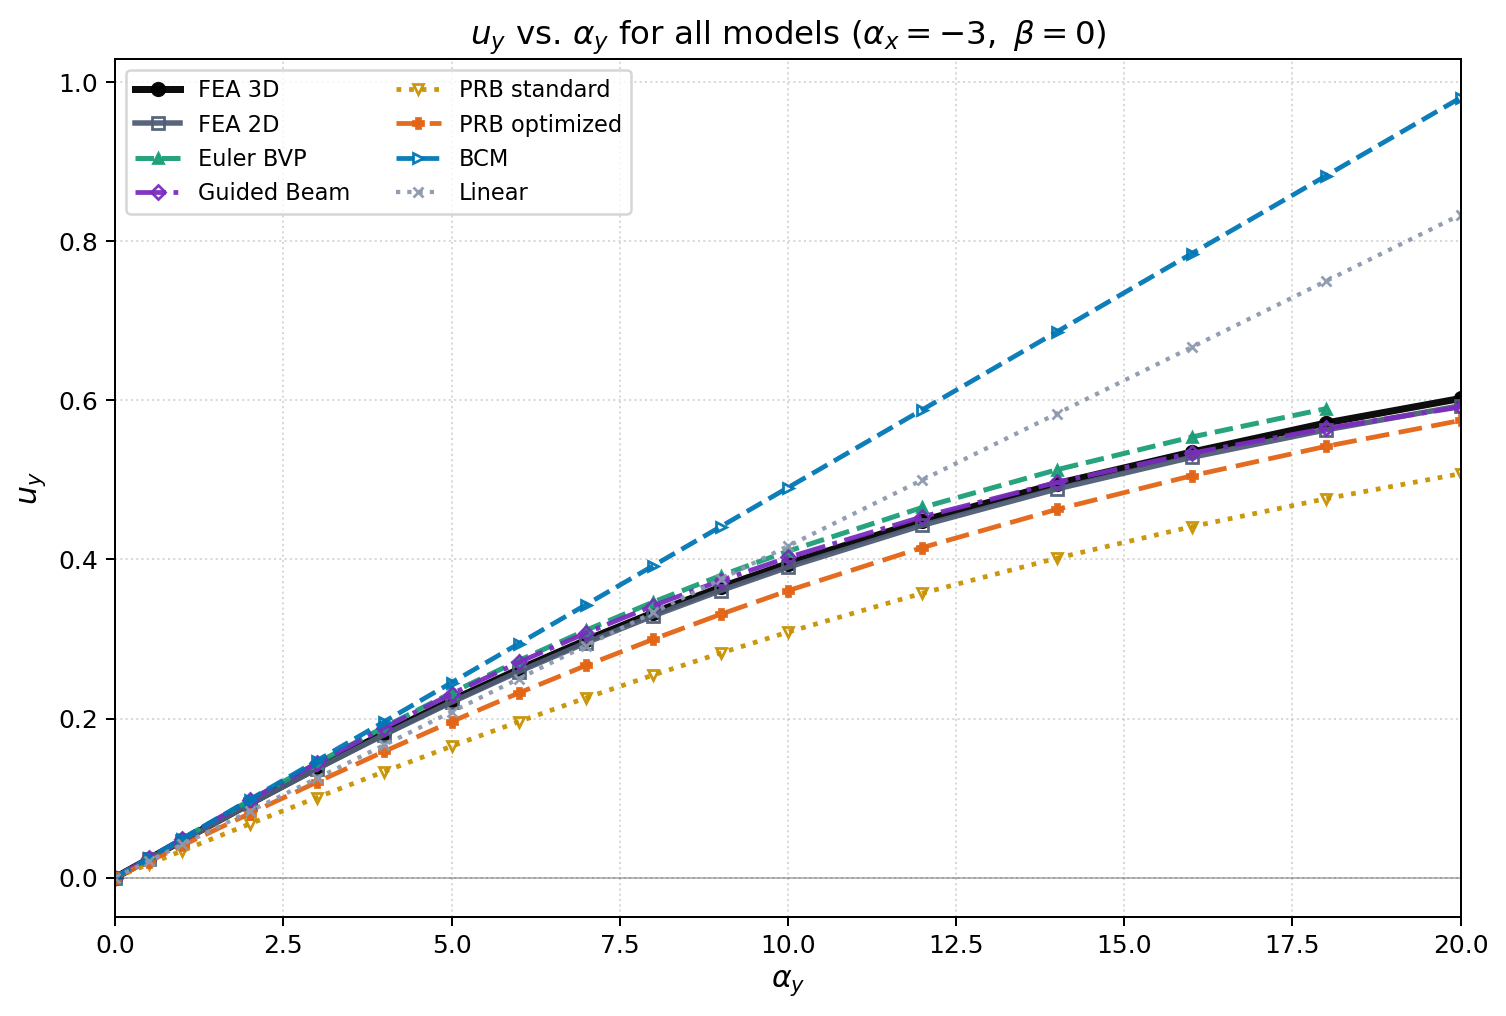
\includegraphics[width=0.95\columnwidth]{images/uy_vs_Ay_all_models_Ax_neg3_B0.png}
        \caption{$u_y$ vs. $\alpha_y$}
    \end{subfigure}
    \vspace{0.3cm}
    \begin{subfigure}[b]{\columnwidth}
        \centering
        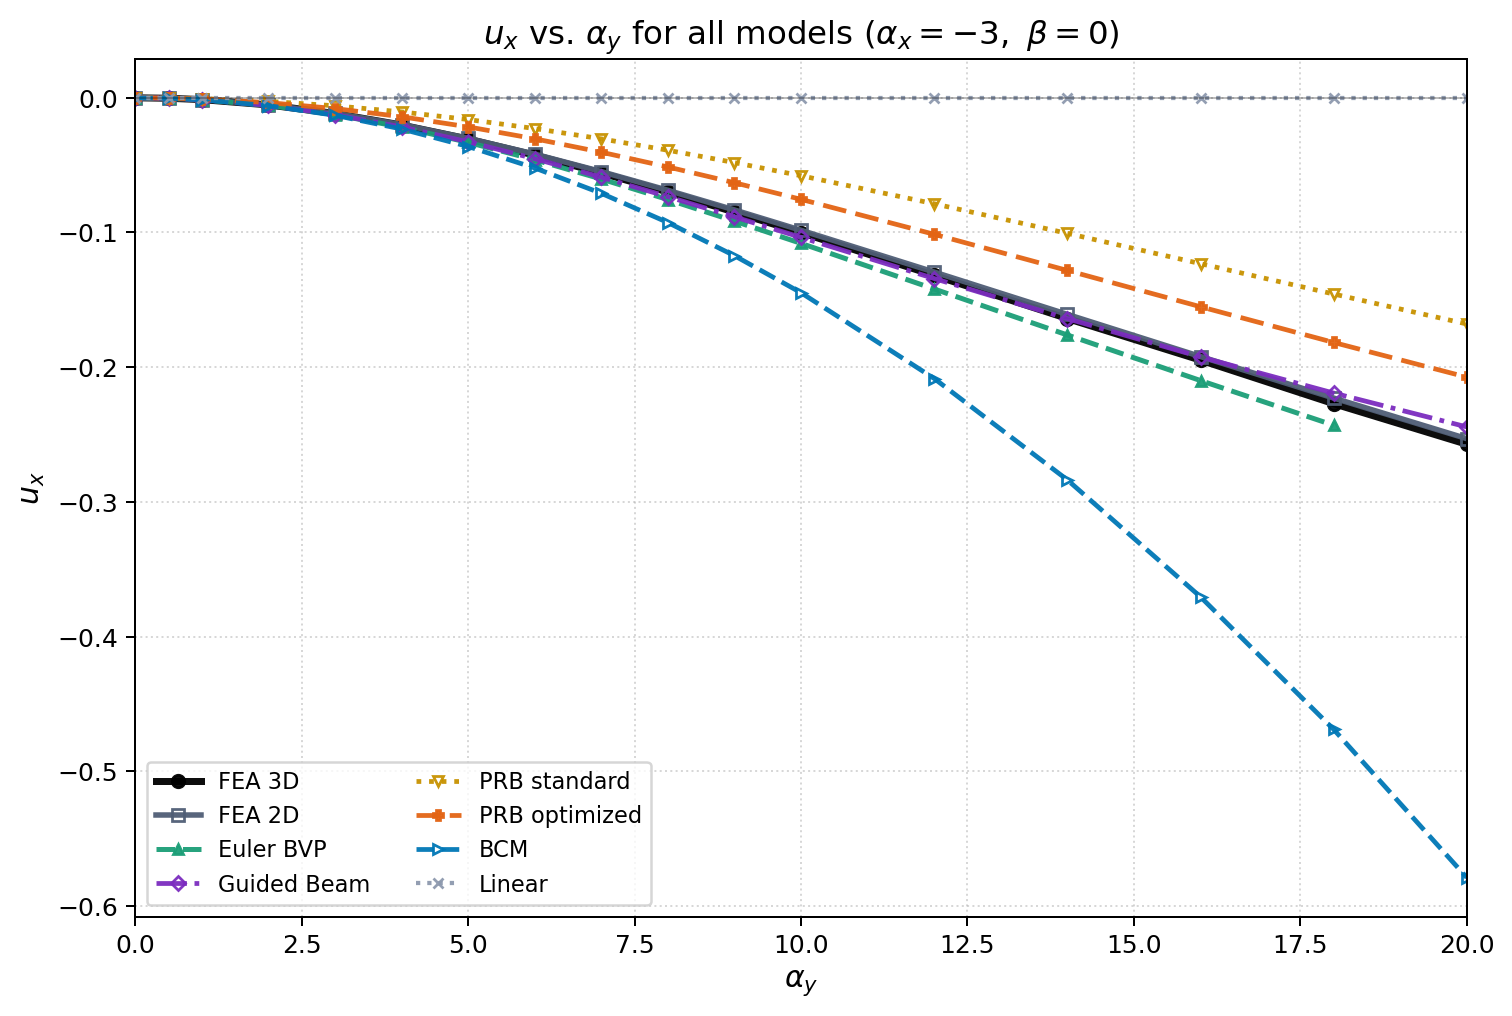
\includegraphics[width=0.95\columnwidth]{images/ux_vs_Ay_all_models_Ax_neg3_B0.png}
        \caption{$u_x$ vs. $\alpha_y$}
    \end{subfigure}
    \vspace{0.3cm}
    \begin{subfigure}[b]{\columnwidth}
        \centering
        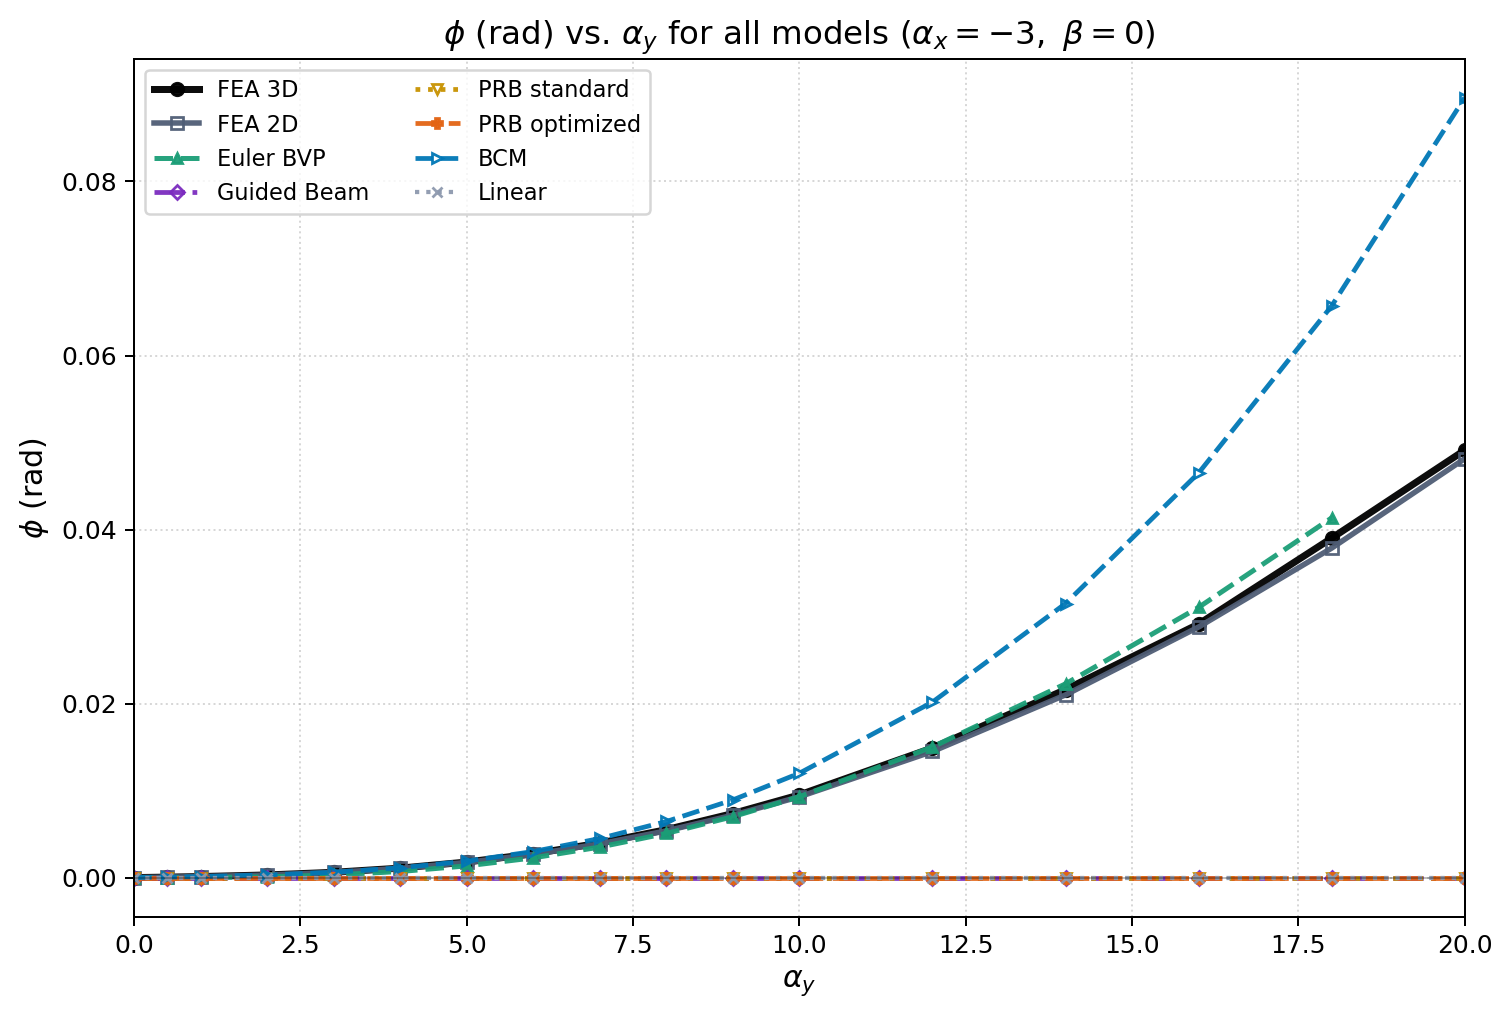
\includegraphics[width=0.95\columnwidth]{images/phi_vs_Ay_all_models_Ax_neg3_B0.png}
        \caption{$\phi$ vs. $\alpha_y$}
    \end{subfigure}
    \caption{Mechanism response under compressive axial loading (\texorpdfstring{$\alpha_x = -3, \beta = 0$}{alpha_x = -3, beta = 0}). The models exhibit significant divergence as the system approaches the buckling limit.}
    \label{fig:case2_accuracy}
\end{figure}

\begin{figure}[ht!]
    \centering
    \begin{subfigure}[b]{\columnwidth}
        \centering
        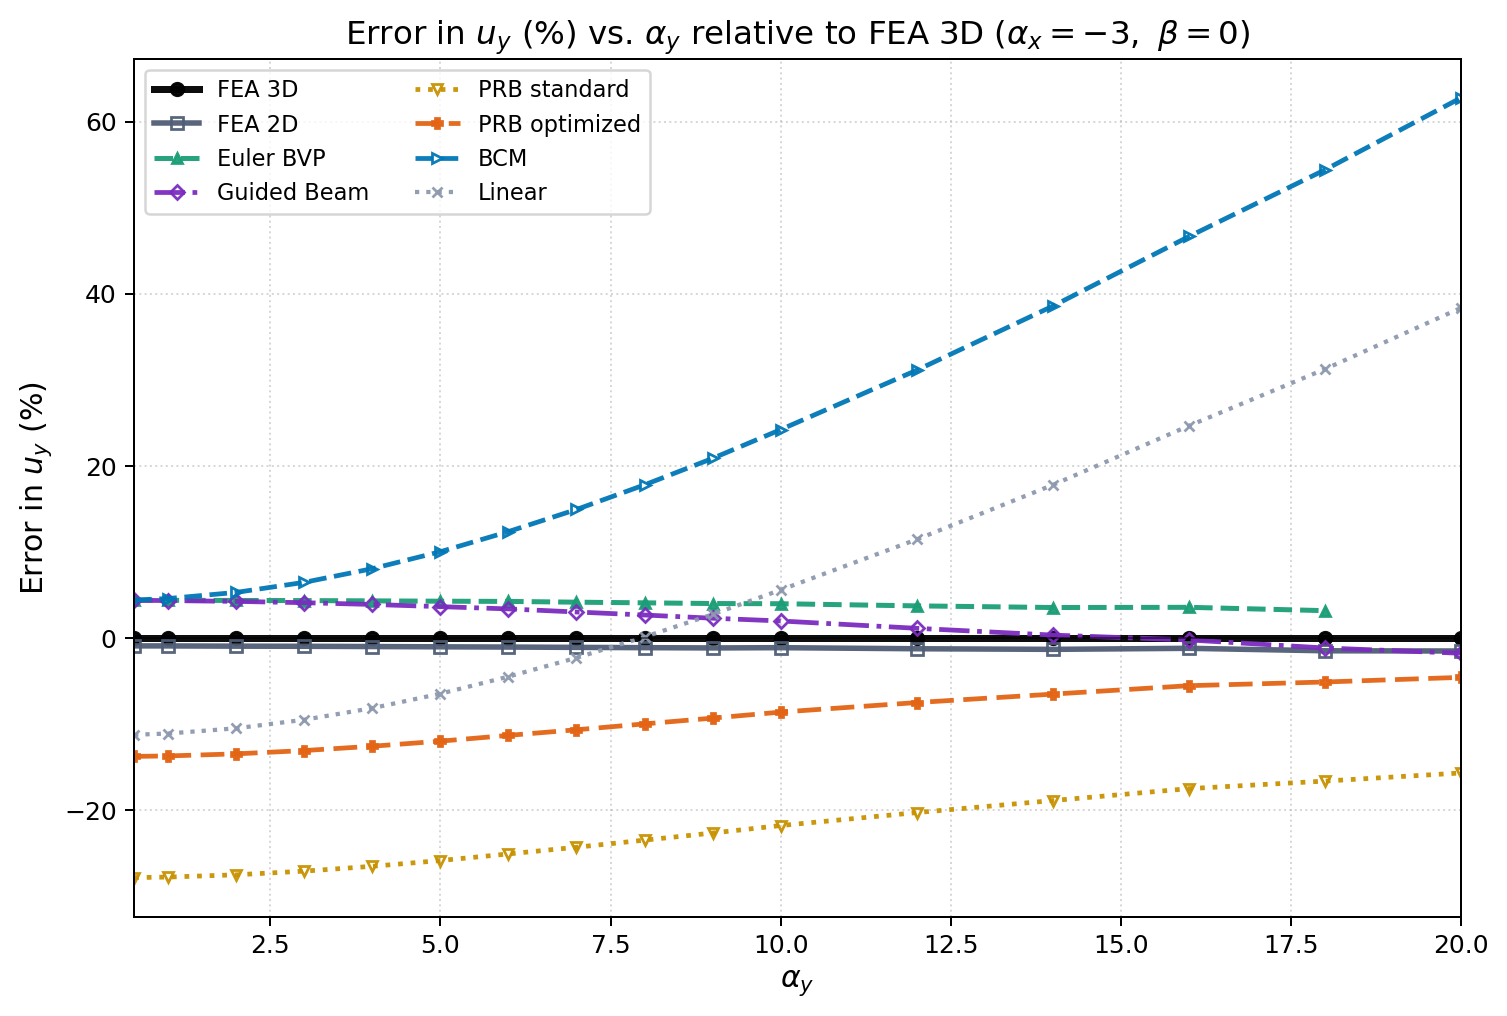
\includegraphics[width=0.95\columnwidth]{images/uy_error_pct_vs_Ay_all_models_Ax_neg3_B0.png}
        \caption{Relative error in $u_y$}
    \end{subfigure}
    \vspace{0.3cm}
    \begin{subfigure}[b]{\columnwidth}
        \centering
        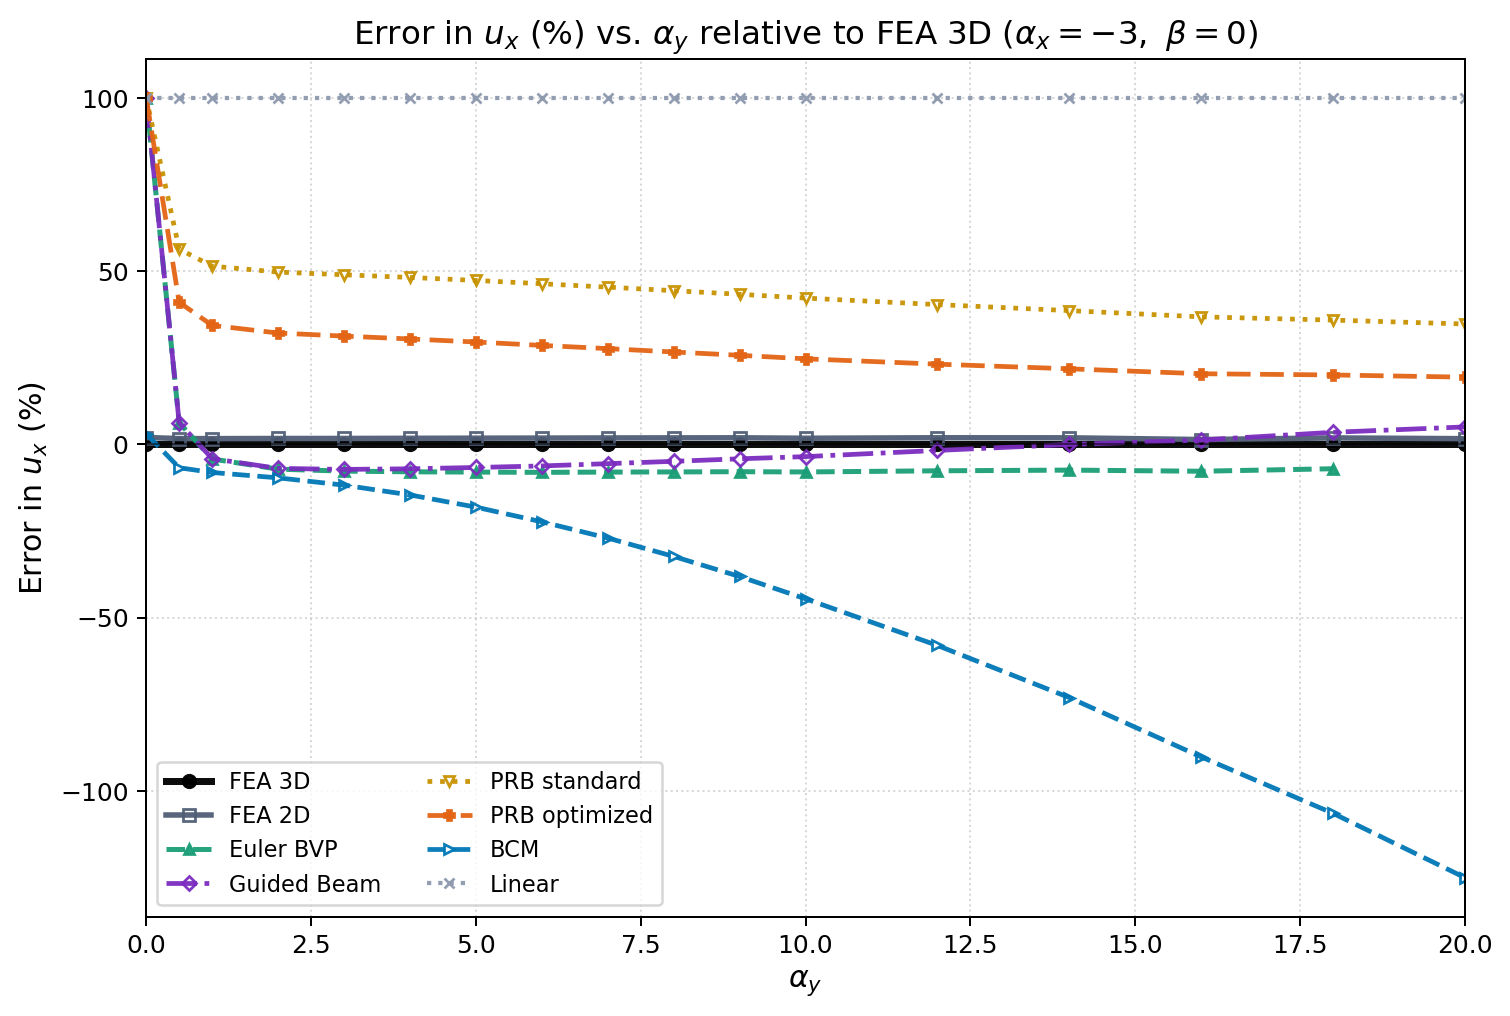
\includegraphics[width=0.95\columnwidth]{images/ux_error_pct_vs_Ay_all_models_Ax_neg3_B0.png}
        \caption{Relative error in $u_x$}
    \end{subfigure}
    \vspace{0.3cm}
    \begin{subfigure}[b]{\columnwidth}
        \centering
        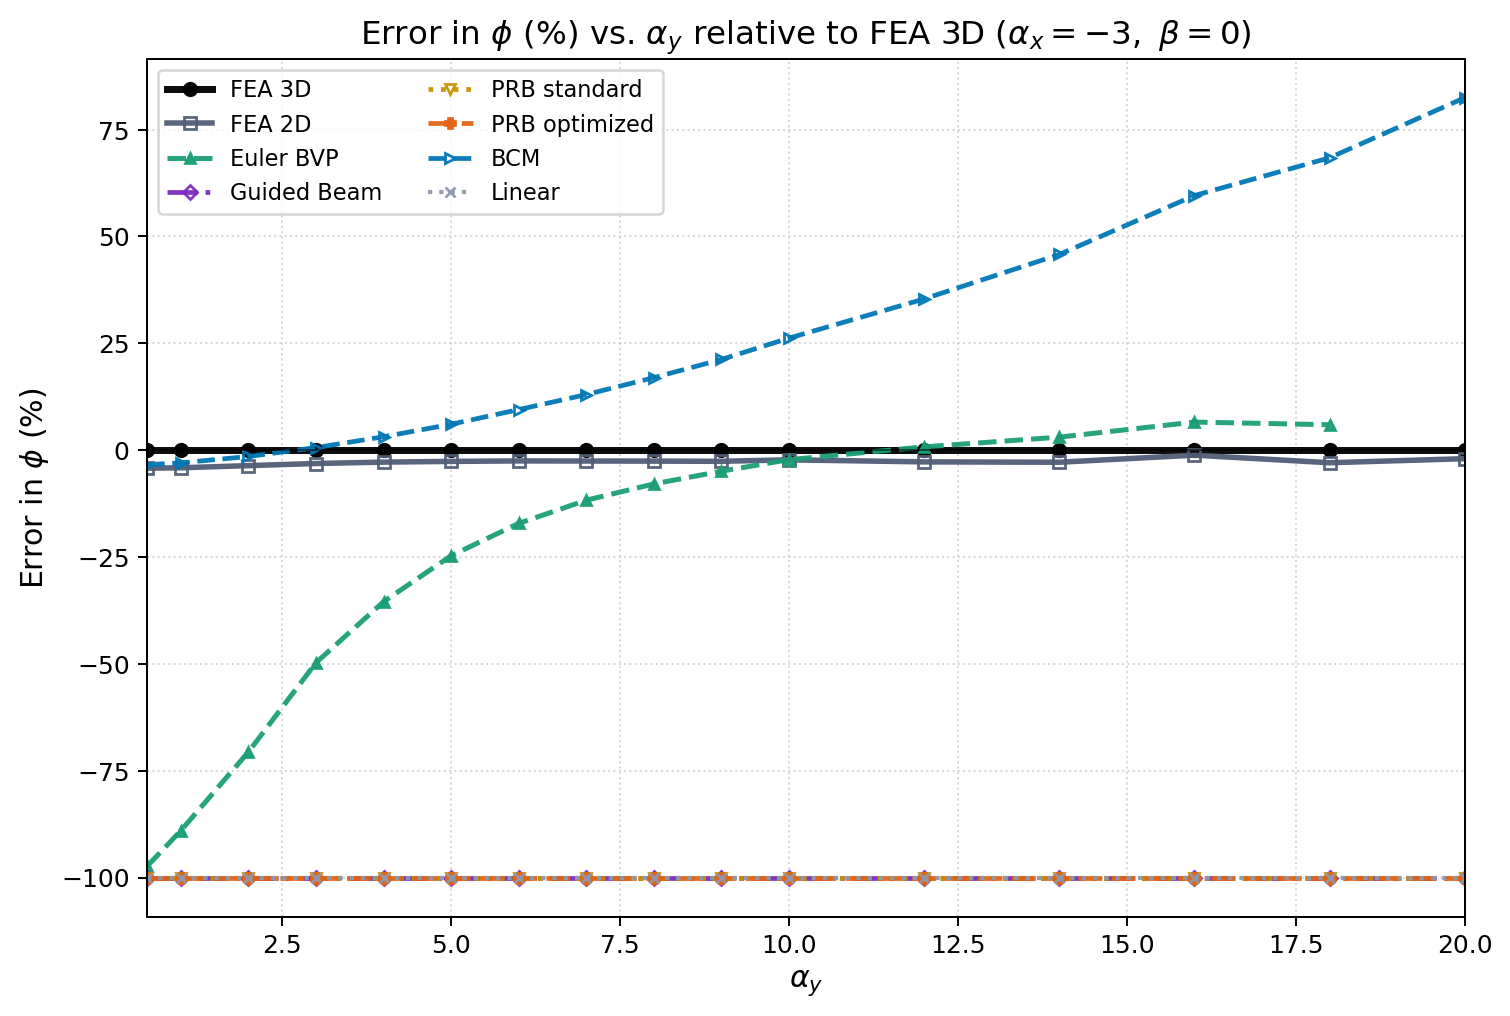
\includegraphics[width=0.95\columnwidth]{images/phi_error_pct_vs_Ay_all_models_Ax_neg3_B0.png}
        \caption{Relative error in $\phi$}
    \end{subfigure}
    \caption{Relative error percentages for modeling levels under compressive axial loading ($\alpha_x = -3, \beta = 0$) relative to the 3D FEA ground truth.}
    \label{fig:case2_errors}
\end{figure}
\section{Results and Discussion}
\label{sec:discussions}

The eight-level modeling stack provides a structured pathway for compliant mechanism design. The BCM offers a "sweet spot" for conceptual design, providing kinematic nonlinearities with O(1) computational complexity. For synthesis tasks requiring optimization over thousands of iterations, the BCM or optimized PRB models are indispensable.

However, high-fidelity verification still requires the Euler BVP or FEA levels. The emergence of parasitic rotation $\phi$, reaching up to $0.4^\circ$ in our nominal benchmark, can be critical in precision metrology applications. Our results confirm that while low-order models capture the primary stiffness, they often fail to predict these second-order geometric couplings, necessitating a validation step using the upper levels of the stack.

\section{Conclusion}
\label{sec:conclusions}

This paper has presented a hierarchical, eight-level multi-fidelity modeling stack for the design and analysis of compliant parallelogram mechanisms. While the parallelogram flexure served as the specific benchmark for this study, the hierarchical organization and the systematic cross-validation of modeling levels constitute a general technical routine applicable to broader classes of compliant mechanisms. By systematically organizing model fidelities from first-order linear theory to high-fidelity 3D solid FEA, we provide a unified framework that bridges the gap between rapid conceptual synthesis and rigorous physical validation. 

The core contributions and findings of this work are summarized as follows:
\begin{enumerate}
    \item \textbf{Validated Hierarchy:} We successfully implemented and cross-validated eight disparate modeling levels, including algebraic (Linear, BCM, PRBM), transcendental (Guided Beam), and numerical (Euler BVP, FEA) approaches. Each level captures progressively more complex phenomenon, from simple stiffness to parasitic rotations and out-of-plane effects.
    \item \textbf{Performance Tradeoffs:} Our runtime analysis demonstrated a performance spread of over eight orders of magnitude. While 3D FEA requires $\sim$44 seconds per load case, the algebraic BCM and Linear models achieve near-instantaneous evaluation ($<10^{-6}$ s), enabling massive-scale design optimization.
    \item \textbf{Optimized PRBM:} We demonstrated that standard PRB parameters often underpredict deflections under high loads. By utilizing an optimized factor ($\gamma = 0.90$) derived from a systematic parametric sweep, we significantly improved the model's accuracy under axial compressive loads without increasing computational complexity.
    \item \textbf{Buckling \& Nonlinear Effects:} Comparative studies (Cases 1 \& 2) highlighted the critical impact of axial loading. While BCM is highly efficient for moderate deflections, its accuracy degrades rapidly near the buckling threshold, where the specialized PRB or BVP models provide more robust performance.
    \item \textbf{Interactive Benchmarking:} The development of an open-source interactive app and a public dataset of over 3,000 load cases provides the community with a baseline for future multi-fidelity research.
\end{enumerate}

Future work will focus on integrating these disparate modeling levels into a single, adaptive framework that automatically switches between fidelities based on real-time assessments of required computational efficiency, predictive accuracy, and deformation scale. Furthermore, the generated dataset of over 3,000 load cases provides a robust foundation for training specialized machine learning models dedicated to the rapid design synthesis of compliant parallelogram mechanisms. Such models could facilitate instantaneous synthesis while satisfying stringent industry requirements for both efficiency and accuracy across large workspaces. Additionally, this hierarchical stack serves as an ideal basis for physics-informed machine learning (PINN) surrogates, where analytical models provide the physical priors for high-fidelity data-driven refinement.




%%%%% Acknowledgments %%%%%%%%%%%%%%%%%%%%%%%%%%%%%%%%%%%

%\section*{Acknowledgments}
%The author acknowledges the use of OpenAI GPT-4 and Anthropic Claude for code generation assistance in this work.


%%%  REFERENCES  %%%%%%%%%%%%%%%%%%%%%%%%%%%%%%%%

\bibliographystyle{asmeconf}
\bibliography{CM_model_stack}

\end{document}
